\documentclass[12pt,a4paper]{article}

% ==============================================================================
% CẤU HÌNH GÓI: 100% PDFLATEX TIÊU CHUẨN CHO TIẾNG VIỆT
% ==============================================================================
\usepackage[utf8]{inputenc}
\usepackage[vietnamese,english]{babel}
\usepackage[T5]{fontenc}
\usepackage{lmodern}
\usepackage[margin=1.8cm,top=2.5cm,bottom=2.2cm,headheight=24pt]{geometry}
\usepackage{amsmath,amssymb}
\usepackage{booktabs}
\usepackage{graphicx}
\usepackage{hyperref}
\usepackage{fancyhdr}
\usepackage{cite}
\usepackage{tabularx}
\usepackage{chngcntr}
\usepackage{xcolor}

% Điều chỉnh độ dãn dòng và chống tràn lề
\emergencystretch=1.5em

% Đánh số phương trình, bảng biểu, hình vẽ theo từng Section (ví dụ: Hình 2.1, Bảng 2.1)
\counterwithin{table}{section}
\counterwithin{figure}{section}
\counterwithin{equation}{section}

% Cấu hình liên kết Hyperref
\hypersetup{
    colorlinks=true,
    linkcolor=blue!80!black,
    citecolor=blue!70!black,
    urlcolor=blue!80!black,
    plainpages=false
}

% Cấu hình Header và Footer theo mẫu chuẩn của Khoa KH&KT Máy tính - ĐH Bách khoa
\pagestyle{fancy}
\fancyhf{}
\setlength{\headheight}{24pt}
\fancyhead[L]{\fontsize{8.5}{10.5}\selectfont \textbf{ĐẠI HỌC BÁCH KHOA -- ĐHQG TP. HỒ CHÍ MINH}\\
\textbf{KHOA KHOA HỌC VÀ KỸ THUẬT MÁY TÍNH}}
\fancyhead[R]{\fontsize{8.5}{10.5}\selectfont \textbf{CO3133 -- BÁO CÁO TIẾN ĐỘ SỐ 3}\\
\textit{Học kỳ I / Năm học 2026--2027}}
\renewcommand{\headrulewidth}{0.5pt}
\fancyfoot[L]{\fontsize{8.5}{10.5}\selectfont \textit{Dự án Doanh nghiệp HK261-DAGD1-558}}
\fancyfoot[R]{\fontsize{8.5}{10.5}\selectfont \textbf{Trang \thepage}}
\renewcommand{\footrulewidth}{0.4pt}

\begin{document}
\selectlanguage{vietnamese}

% ==============================================================================
% TRANG BÌA CHUẨN KHOA KHOA HỌC VÀ KỸ THUẬT MÁY TÍNH
% ==============================================================================
\begin{titlepage}
\hypersetup{pageanchor=false}
\centering
{\bfseries\large ĐẠI HỌC QUỐC GIA THÀNH PHỐ HỒ CHÍ MINH\\[3pt]
TRƯỜNG ĐẠI HỌC BÁCH KHOA\\[3pt]
KHOA KHOA HỌC VÀ KỸ THUẬT MÁY TÍNH\par}
\vspace{1.2cm}

% Biểu trưng Khoa / Trường
\IfFileExists{HCMUT-logo.png}{
    
\includegraphics[width=3.2cm]{HCMUT-logo.png}
}{
    \framebox[3.2cm]{\rule{0pt}{3.2cm} \textbf{BK TP.HCM}}
}

\vspace{1.2cm}
{\Large\bfseries BÁO CÁO TIẾN ĐỘ TUẦN (SỐ 03)\par}
\vspace{0.25cm}
{\large Học kỳ Doanh nghiệp (HK261) \quad\textbar\quad Kỳ báo cáo: 12/10 -- 25/10/2026\par}
\vspace{0.8cm}

\rule{\linewidth}{1.2pt}\\[0.4cm]
{\Large\bfseries PHÁT TRIỂN HỆ THỐNG PHÂN ĐOẠN THỰC THỂ VÀ ĐỊNH VỊ 3D MỤC TIÊU SẦU RIÊNG DỰA TRÊN YOLOV8-SEG VÀ CẢM BIẾN ĐỘ SÂU CHO ROBOT NÔNG NGHIỆP TỰ HÀNH\par}
\vspace{0.2cm}
\rule{\linewidth}{1.2pt}

\vspace{0.6cm}
{\large\bfseries Môn học: Học sâu và Ứng dụng (CO3133)\par}
\vspace{0.2cm}
{\normalsize Dự án Doanh nghiệp gốc: \textbf{HK261-DAGD1-558}\par}
{\footnotesize (Nâng cấp và Tự chủ Công nghệ Robot Nông nghiệp Tự hành cho UGV Phun thuốc có Tháp pháo 2 trục trên Địa hình Đồi dốc)\par}

\vspace{1.2cm}
\begin{flushleft}
\large
\begin{tabular}{@{}ll@{}}
\textbf{Giảng viên hướng dẫn:} & \textbf{ThS. Nguyễn Quốc Minh} \\
                              & Bộ môn Khoa học Máy tính, Khoa KH\&KT Máy tính \\[0.3cm]
\textbf{Sinh viên thực hiện:}  & \textbf{Trần Hữu Hoàng Long} \quad (MSSV: \textbf{2352704}) \\
                              & \textbf{Trương Gia Hy} \quad\quad\quad (MSSV: \textbf{2352458}) \\[0.3cm]

\end{tabular}
\end{flushleft}

\vfill
{\large Thành phố Hồ Chí Minh, Tháng 10 năm 2026\par}
\end{titlepage}
\hypersetup{pageanchor=true}

% ==============================================================================
% PHẦN ĐẦU: ÁNH XẠ CHUẨN ĐẦU RA VÀ MỤC LỤC
% ==============================================================================
\newpage
\pagenumbering{roman}

\section*{Bảng tổng kết đáp ứng Chuẩn đầu ra (CĐR) môn học}
\addcontentsline{toc}{section}{Bảng tổng kết đáp ứng Chuẩn đầu ra (CĐR) môn học}

Báo cáo tiến độ này tuân thủ các Chuẩn đầu ra (CĐR) cốt lõi của đề cương môn học \textbf{CO3133: Học sâu và Ứng dụng} thuộc Khoa Khoa học và Kỹ thuật Máy tính -- Trường Đại học Bách khoa, ĐHQG-HCM. Bảng~\ref{tab:cdr_front_mapping} tổng hợp sự ánh xạ giữa các kết quả kỹ thuật đã hoàn thành trong giai đoạn này và các chỉ số đo lường học phần tương ứng.

\begin{table}[htbp]
\centering
\small
\caption{Bảng ánh xạ các kết quả bàn giao của Sprint 3 với Chuẩn đầu ra môn CO3133.}
\label{tab:cdr_front_mapping}
\begin{tabularx}{\textwidth}{l p{3.8cm} X c}
\toprule
\textbf{Chuẩn đầu ra} & \textbf{Định nghĩa theo Đề cương} & \textbf{Minh chứng thực nghiệm trong Báo cáo} & \textbf{Trạng thái} \\
\midrule
\textbf{CĐR 8 (L.O.5.1)} & Đánh giá thực nghiệm các mô hình học sâu qua bảng ablation, loss curve, confusion matrix và kiểm định thống kê. & Thực hiện benchmark định lượng 5 kịch bản trên GPU RTX 3060 (Bảng~2.1), phân tích hội tụ hàm mất mát đa nhiệm (Hình~2.1), giải thích cú nảy gradient ngắt Mosaic tại Epoch 20, phân rã lỗi ma trận nhầm lẫn và ước lượng khoảng tin cậy Wilson 95\% cho Recall. & \textbf{Đã hoàn thành} \\
\addlinespace
\textbf{CĐR 9 (L.O.5.2)} & Phân tích các đánh đổi kỹ thuật (độ chính xác, độ trễ, bộ nhớ, nhiệt độ) để lựa chọn mô hình triển khai thực tế. & Phân tích mở rộng kiến trúc YOLOv8n-seg so với YOLOv8s-seg (Mục~3.1), đánh đổi độ phân giải và kích thước batch, phân bổ ngân sách bộ nhớ và tính toán trên kit nhúng Raspberry Pi 5 (16\,GB), phối hợp cùng cảm biến Intel RealSense D453i và LiDAR C1M1. & \textbf{Đã hoàn thành} \\
\addlinespace
\textbf{CĐR 4 (L.O.4.1)} & Hiện thực, huấn luyện và đánh giá mô hình học sâu trên trạm tính toán GPU chuyên dụng. & Vận hành pipeline huấn luyện trên trạm GPU NVIDIA RTX 3060 sử dụng PyTorch 2.3.0 và Ultralytics 8.2 trên tập 2,676 ảnh gán nhãn đa giác sầu riêng. & \textbf{Đã hoàn thành} \\
\addlinespace
\textbf{CĐR 5 (L.O.4.2)} & Thu thập, tiền xử lý, tăng cường và kiểm toán dữ liệu để đảm bảo tính nhất quán và chống rò rỉ dữ liệu. & Gộp dữ liệu từ 5 kho Roboflow, chuẩn hóa về lớp sầu riêng duy nhất, đưa tọa độ đa giác về $[0, 1]$, chia tập độc lập 80/14/6 và áp dụng tăng cường trực tuyến (online augmentation) trong bộ nhớ. & \textbf{Đã hoàn thành} \\
\bottomrule
\end{tabularx}
\end{table}

\newpage
\vspace{0.4cm}
\tableofcontents
\vspace{0.4cm}
\listoftables
\vspace{0.4cm}
\listoffigures

\newpage
\pagenumbering{arabic}

% ==============================================================================
% MỤC 1: BỐI CẢNH DỰ ÁN VÀ KHỞI ĐỘNG
% ==============================================================================
\section{Bối cảnh dự án và khởi động (Project Kickoff)}

\subsection{Mục tiêu và động lực kỹ thuật}
Trong canh tác nông nghiệp công nghệ cao tại các vùng địa hình đồi dốc và ruộng bậc thang, sầu riêng (\textit{Durio zibethinus}) là loại cây ăn trái có giá trị kinh tế đặc biệt lớn nhưng đòi hỏi quy trình chăm sóc và bảo vệ thực vật nghiêm ngặt. Cây sầu riêng rất mẫn cảm với bệnh xì mủ thối thân và thối quả do nấm \textit{Phytophthora palmivora} gây ra. Việc phun thuốc bảo vệ thực vật thủ công bằng tay trên các sườn dốc hiểm trở tiềm ẩn rủi ro trượt ngã, ngộ độc hóa chất cho người lao động và hiệu quả bao phủ không đồng đều.

Dưới sự tài trợ của Dự án Doanh nghiệp mã số \textbf{HK261-DAGD1-558}, đề tài của nhóm tập trung phát triển hệ thống thị giác máy tính thông minh hướng dẫn ngắm bắn mục tiêu thời gian thực cho phương tiện tự hành mặt đất (Unmanned Ground Vehicle -- UGV). Robot nông nghiệp được tích hợp một cảm biến thu nhận hình ảnh RGB-D và một tháp pháo phun thuốc 2 trục (dual-axis pan-tilt spraying turret). Robot có nhiệm vụ tự hành men theo các hàng cây, nhận diện từng quả sầu riêng đang treo trên tán lá và điều khiển góc quay pan-tilt của vòi phun áp lực cao bắn chính xác vào tâm quả.

\paragraph{Cơ sở khoa học cho việc chuyển dịch từ Bounding Box 2D sang Phân đoạn thực thể (Instance Segmentation):}
Trong các nghiên cứu robot nông nghiệp truyền thống, việc phát hiện quả thường dựa vào mô hình nhận diện 2D dạng hộp bao chữ nhật (Bounding Box) $[x_{\min}, y_{\min}, x_{\max}, y_{\max}]$. Tuy nhiên, nhiều công trình tổng quan và thực nghiệm uy tín trên tạp chí \textit{Computers and Electronics in Agriculture} đã chỉ ra những hạn chế cố hữu của phương pháp này:
\begin{itemize}
    \item \textbf{Nhiễm bẩn chiều sâu từ hậu cảnh và tiền cảnh (Depth Contamination / Bleeding):} Fu và cộng sự \cite{fu2020rgbd} trong bài tổng quan toàn diện về ứng dụng camera RGB-D trên robot thu hoạch đã chỉ ra rằng hộp bao chữ nhật luôn chứa một lượng lớn điểm ảnh không thuộc về quả. Khi lấy mẫu độ sâu tại tâm hình học $(u_c, v_c)$ hoặc tính trung bình cộng trong hộp bao, tia đo rất dễ rơi vào các kẽ lá hở nhìn xuyên ra hậu cảnh xa (Background Bleeding) hoặc trúng vào các cành lá nằm chắn ở tiền cảnh phía trước quả (Foreground Occlusion Bleeding).
    \item \textbf{Sai lệch định vị không gian 3D:} Lin và cộng sự \cite{lin2021fruit} cùng Kang \& Chen \cite{kang2020dasnet} đã chứng minh thực nghiệm rằng việc sử dụng mặt nạ phân đoạn thực thể cấp điểm ảnh (pixel-level instance segmentation) là điều kiện tiên quyết để bóc tách chính xác ranh giới hình thái quả, loại bỏ hoàn toàn các điểm ảnh cành lá xung quanh trước khi chiếu ngược sang hệ trục tọa độ 3D, giúp giảm triệt để sai số bám mục tiêu của cơ cấu chấp hành.
\end{itemize}

\paragraph{Giải pháp đề xuất --- Khung giải thuật MF-3DLoc:}
Kể từ sự ra đời của Mask R-CNN \cite{he2017maskrcnn} và các mạng phân đoạn một giai đoạn thời gian thực như YOLACT \cite{bolya2019yolact} hay YOLOv8-Seg \cite{ultralytics2023}, việc phân đoạn thực thể cấp điểm ảnh đã trở thành tiêu chuẩn vàng để nhận diện nông sản chính xác. Kế thừa các kết luận khoa học trên, nhóm đề xuất giải thuật \textbf{MF-3DLoc (Mask-Filtered 3D Localization)}. MF-3DLoc sử dụng mạng nơ-ron tích chập YOLOv8-Seg \cite{ultralytics2023} để dự đoán mặt nạ phân đoạn thực thể nhị phân $M(u, v) \in \{0, 1\}$ ôm sát vỏ quả gai. Bằng cách sử dụng mặt nạ này làm bộ lọc không gian (spatial gating), thuật toán cô lập strictly các điểm ảnh thuộc về bề mặt quả và áp dụng toán tử lọc trung vị (Median filter với điểm phá vỡ tối đa 50\%), loại bỏ hoàn toàn hiện tượng depth bleeding từ cành lá phụ cận trước khi giải phương trình chiếu ngược Pinhole để tính toán vectơ tọa độ 3D $(X, Y, Z)$ cấp cho bộ điều khiển tháp pháo.
\subsection{Môi trường thực nghiệm và Thông số kỹ thuật}
Toàn bộ quá trình huấn luyện mô hình, đo đạc thông lượng và phân tích thống kê được thực hiện trên máy tính để bàn với cấu hình xác thực như sau:
\begin{itemize}
    \item \textbf{Bộ vi xử lý trung tâm (CPU):} 13th Gen Intel Core i5-13400F (10 nhân: 6 P-cores + 4 E-cores, 16 luồng, xung nhịp tối đa 4.60\,GHz);
    \item \textbf{Bộ nhớ trong (RAM):} 32\,GB;
    \item \textbf{Card đồ họa máy trạm (GPU):} NVIDIA GeForce RTX 3060 với 12\,GB GDDR6 VRAM;
    \item \textbf{Hệ điều hành \& Môi trường:} Windows 11 64-bit, CUDA 12.x, PyTorch 2.3.0, Ultralytics 8.2.0;
    \item \textbf{Phần cứng robot nhúng mục tiêu:} Máy tính nhúng Raspberry Pi 5 (bản 16\,GB RAM), cảm biến độ sâu Intel RealSense D453i và cảm biến LiDAR C1M1.
\end{itemize}

% ==============================================================================
% MỤC 2: ĐÁNH GIÁ THỰC NGHIỆM VÀ BENCHMARK ĐỊNH LƯỢNG
% ==============================================================================
\section{Đánh giá thực nghiệm và Benchmark định lượng (Trọng tâm CĐR 8)}

\subsection{Tổng hợp dữ liệu, làm sạch và khử trùng lặp (Deduplication)}
Để mạng phân đoạn thực thể có khả năng tổng quát hóa tốt dưới điều kiện ánh sáng tự nhiên thay đổi, các giống quả khác nhau và độ rậm rạp của tán cây, nhóm đã tổng hợp và chuẩn hóa dữ liệu từ 5 kho lưu trữ Roboflow mở về sầu riêng:
\begin{enumerate}
    \item \texttt{durian-udang-merah} (Tập ảnh sầu riêng giống Udang Merah / Red Prawn);
    \item \texttt{durian-puyat-variety-detector} (Ảnh tán cây sầu riêng giống Puyat);
    \item \texttt{durian-dataset-2} (Ảnh chụp vườn sầu riêng trong điều kiện ánh sáng hỗn hợp);
    \item \texttt{durian-groove-grading} (Ảnh cự ly gần thể hiện chi tiết rãnh và gai vỏ);
    \item \texttt{do-an-tot-nghiep-kuz1c} (Ảnh chụp thu hoạch thực địa dưới ánh nắng ban ngày).
\end{enumerate}

\paragraph{Chuẩn hóa và Tiền xử lý dữ liệu (Dataset Harmonization \& Preprocessing):}
Toàn bộ dữ liệu thu thập từ 5 kho lưu trữ Roboflow được hợp nhất và chuẩn hóa thông qua script chuyên dụng: giải nén các tập dữ liệu, ánh xạ toàn bộ các nhãn lớp về một lớp duy nhất là sầu riêng (\texttt{durian}, class index 0). Tọa độ nhãn đa giác (polygon coordinates) được đưa về dải tương đối $[0, 1]$, xử lý chuyển đổi các nhãn hộp bao 4 góc về định dạng đa giác tương thích, đồng thời sàng lọc và loại bỏ các dòng nhãn suy biến hoặc sai định dạng để bảo đảm chất lượng đầu vào cho mạng phân đoạn.

Tập dữ liệu sạch tổng hợp bao gồm \textbf{2,676 ảnh chất lượng cao} với nhãn phân đoạn đa giác 1:1 bao sát viền gai của từng quả sầu riêng. Tập dữ liệu được phân chia độc lập thành 3 tập con:
\begin{itemize}
    \item \textbf{Tập huấn luyện (Train set):} 2,129 ảnh (chiếm 79.56\% $\approx 80\%$), áp dụng tăng cường trực tuyến;
    \item \textbf{Tập kiểm định (Validation set):} 379 ảnh (chiếm 14.16\% $\approx 14\%$), dùng theo dõi loss và chọn siêu tham số;
    \item \textbf{Tập kiểm thử (Test set):} 168 ảnh (chiếm 6.28\% $\approx 6\%$), được giữ nguyên bản tuyệt đối để đánh giá cuối.
\end{itemize}

\paragraph{Chiến lược tăng cường dữ liệu trực tuyến (Online Augmentation):}
Trong quá trình huấn luyện, các kỹ thuật tăng cường dữ liệu trực tuyến (online data augmentation) được kích hoạt và thực thi tự động trong bộ nhớ GPU bởi chính framework Ultralytics theo từng mini-batch (bao gồm kỹ thuật ghép ảnh 4 góc Mosaic, nhiễu không gian màu HSV, lật ngẫu nhiên và biến đổi tỷ lệ affine). Các phép tăng cường này diễn ra hoàn toàn trên bộ nhớ đệm GPU khi nạp batch mà không tạo ra các tệp ảnh tĩnh trùng lặp trên ổ đĩa. Ngược lại, tập kiểm định (validation) và tập kiểm thử (test) được giữ nguyên vẹn với kích thước cố định để đảm bảo tính khách quan của phép đo.

\subsection{Hàm mất mát đa nhiệm và Động lực học ngắt Mosaic}
Kiến trúc YOLOv8-Seg tối ưu hóa đồng thời 4 thành phần mất mát thông qua một hàm mục tiêu đa nhiệm:
\begin{equation}
\mathcal{L}_{\text{total}} = \lambda_{\text{box}} \mathcal{L}_{\text{CIoU}} + \lambda_{\text{dfl}} \mathcal{L}_{\text{DFL}} + \lambda_{\text{cls}} \mathcal{L}_{\text{BCE\_cls}} + \lambda_{\text{seg}} \mathcal{L}_{\text{BCE\_mask}}
\label{eq:total_loss}
\end{equation}
với các trọng số mặc định: $\lambda_{\text{box}} = 7.5$, $\lambda_{\text{dfl}} = 1.5$, $\lambda_{\text{cls}} = 0.5$, và $\lambda_{\text{seg}} = 2.5$.
\begin{itemize}
    \item $\mathcal{L}_{\text{CIoU}}$ là hàm mất mát Complete Intersection over Union \cite{zheng2020ciou}, xử lý đồng thời độ trùng khớp diện tích, khoảng cách tâm chuẩn hóa và sự tương đồng về tỷ lệ khung hình:
    \begin{equation}
    \mathcal{L}_{\text{CIoU}} = 1 - \text{IoU} + \frac{\rho^2(\mathbf{b}, \mathbf{b}^{gt})}{c^2} + \alpha v
    \end{equation}
    trong đó $\mathbf{b}$ và $\mathbf{b}^{gt}$ là tọa độ tâm hộp bao dự đoán và nhãn gốc, $c$ là độ dài đường chéo hộp bao nhỏ nhất chứa cả hai, và $\alpha v$ đo lường tính nhất quán của tỷ lệ khung hình.
    
    \item $\mathcal{L}_{\text{DFL}}$ là hàm mất mát Distribution Focal Loss \cite{li2020generalized}, mô hình hóa tọa độ hộp bao dưới dạng phân phối xác suất liên tục trên các bin rời rạc, giúp mạng nơ-ron nắm bắt độ bất định tại các đường viền gai gồ ghề của sầu riêng:
    \begin{equation}
    \mathcal{L}_{\text{DFL}}(S_i, S_{i+1}) = - \left( (y_{i+1} - y) \log(S_i) + (y - y_i) \log(S_{i+1}) \right)
    \end{equation}
    
    \item $\mathcal{L}_{\text{BCE\_cls}}$ là mất mát cross-entropy nhị phân áp dụng trên các logit dự đoán lớp mục tiêu.
    
    \item $\mathcal{L}_{\text{BCE\_mask}}$ là mất mát cross-entropy nhị phân cấp điểm ảnh được tính giữa mặt nạ tái tạo $\hat{M}(u, v) = \sigma\left(\sum_{k=1}^{32} w_k P_k(u, v)\right)$ (kết hợp tuyến tính giữa các prototype của ProtoNet và hệ số mask) với mặt nạ nhãn thực tế $M_{gt}(u, v)$ trong miền $\Omega$:
    \begin{equation}
    \mathcal{L}_{\text{BCE\_mask}} = -\frac{1}{|\Omega|} \sum_{(u,v) \in \Omega} \left[ M_{gt}(u,v) \log \hat{M}(u,v) + (1 - M_{gt}(u,v)) \log (1 - \hat{M}(u,v)) \right]
    \end{equation}
\end{itemize}

\begin{figure}[htbp]
\centering
\IfFileExists{baseline_yolov8n_640_b16_e30_results.png}{
    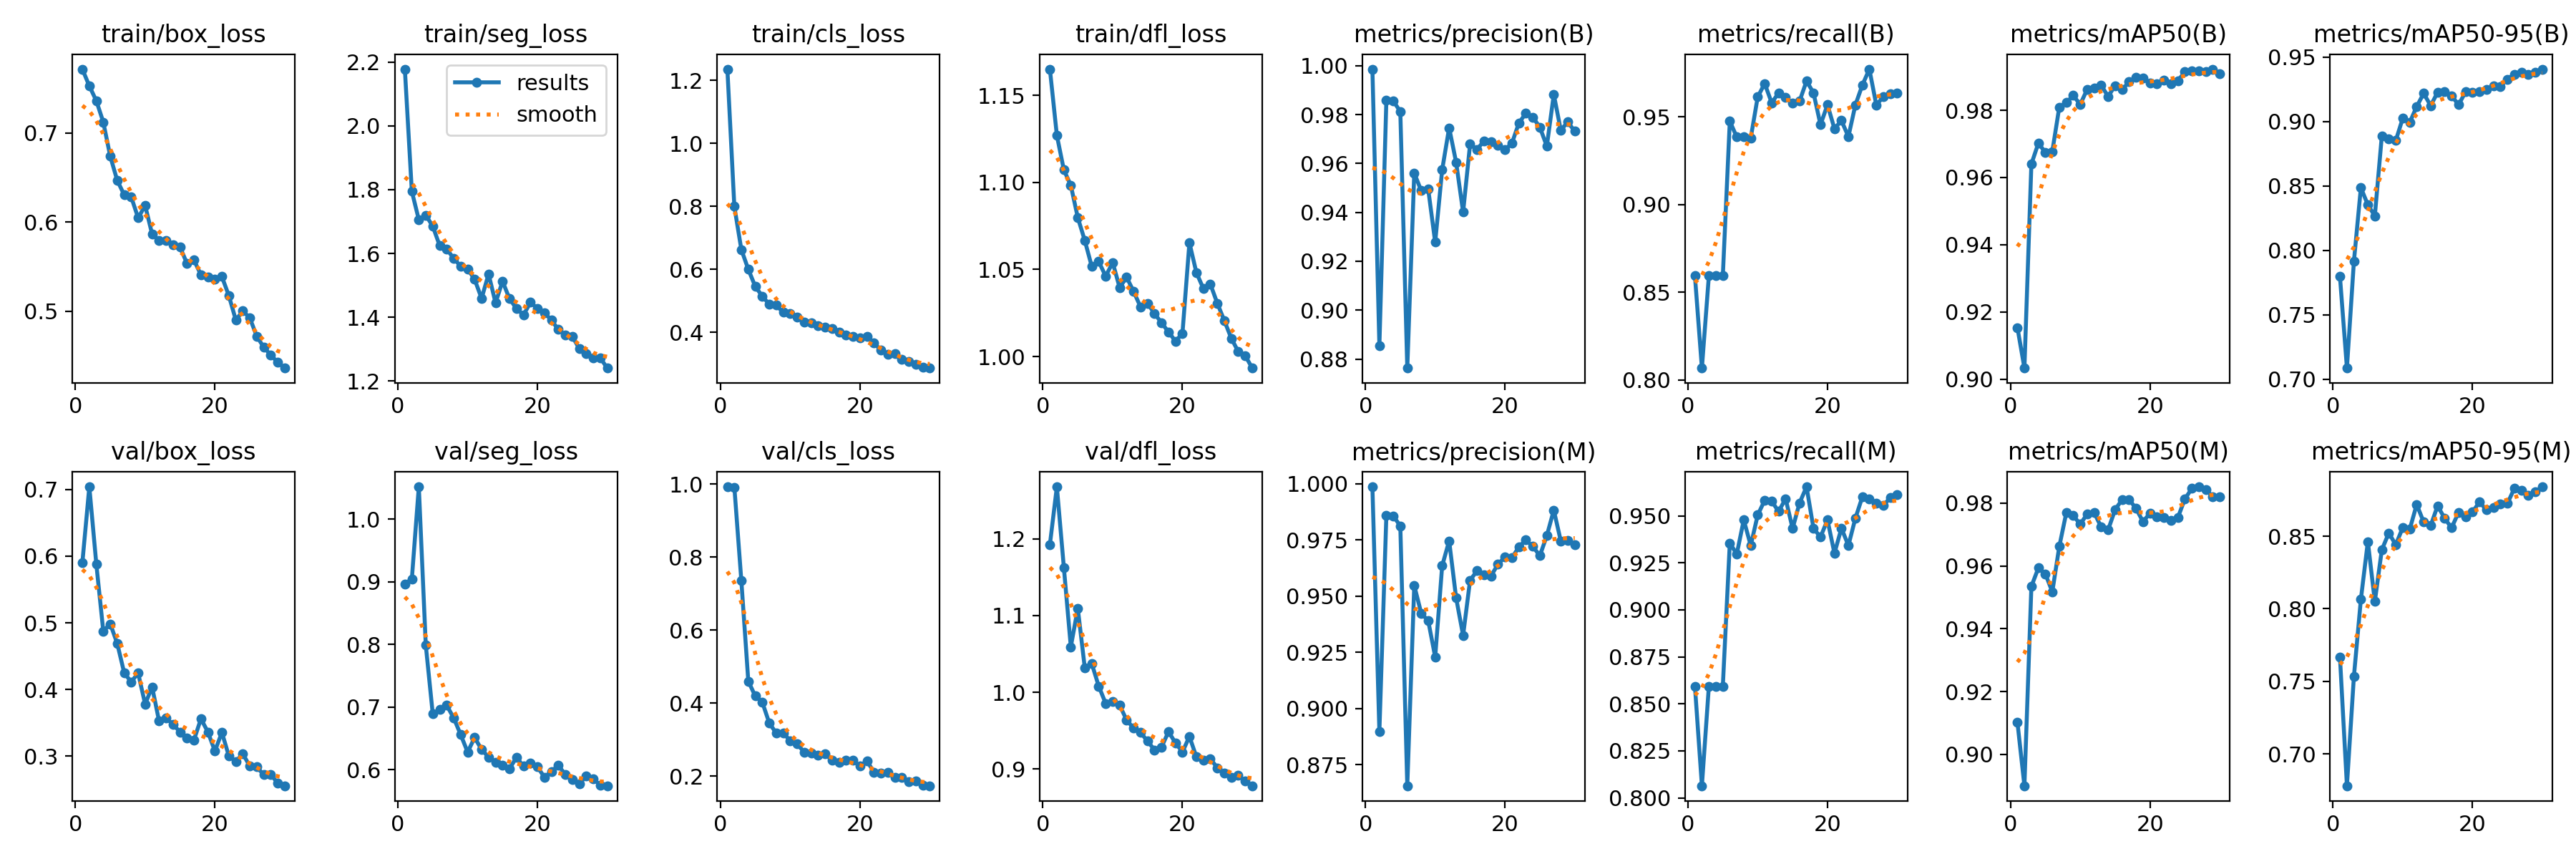
\includegraphics[width=0.95\textwidth]{baseline_yolov8n_640_b16_e30_results.png}
}{
    \IfFileExists{baseline_yolov8n_640_b16_e30_results.jpg}{
        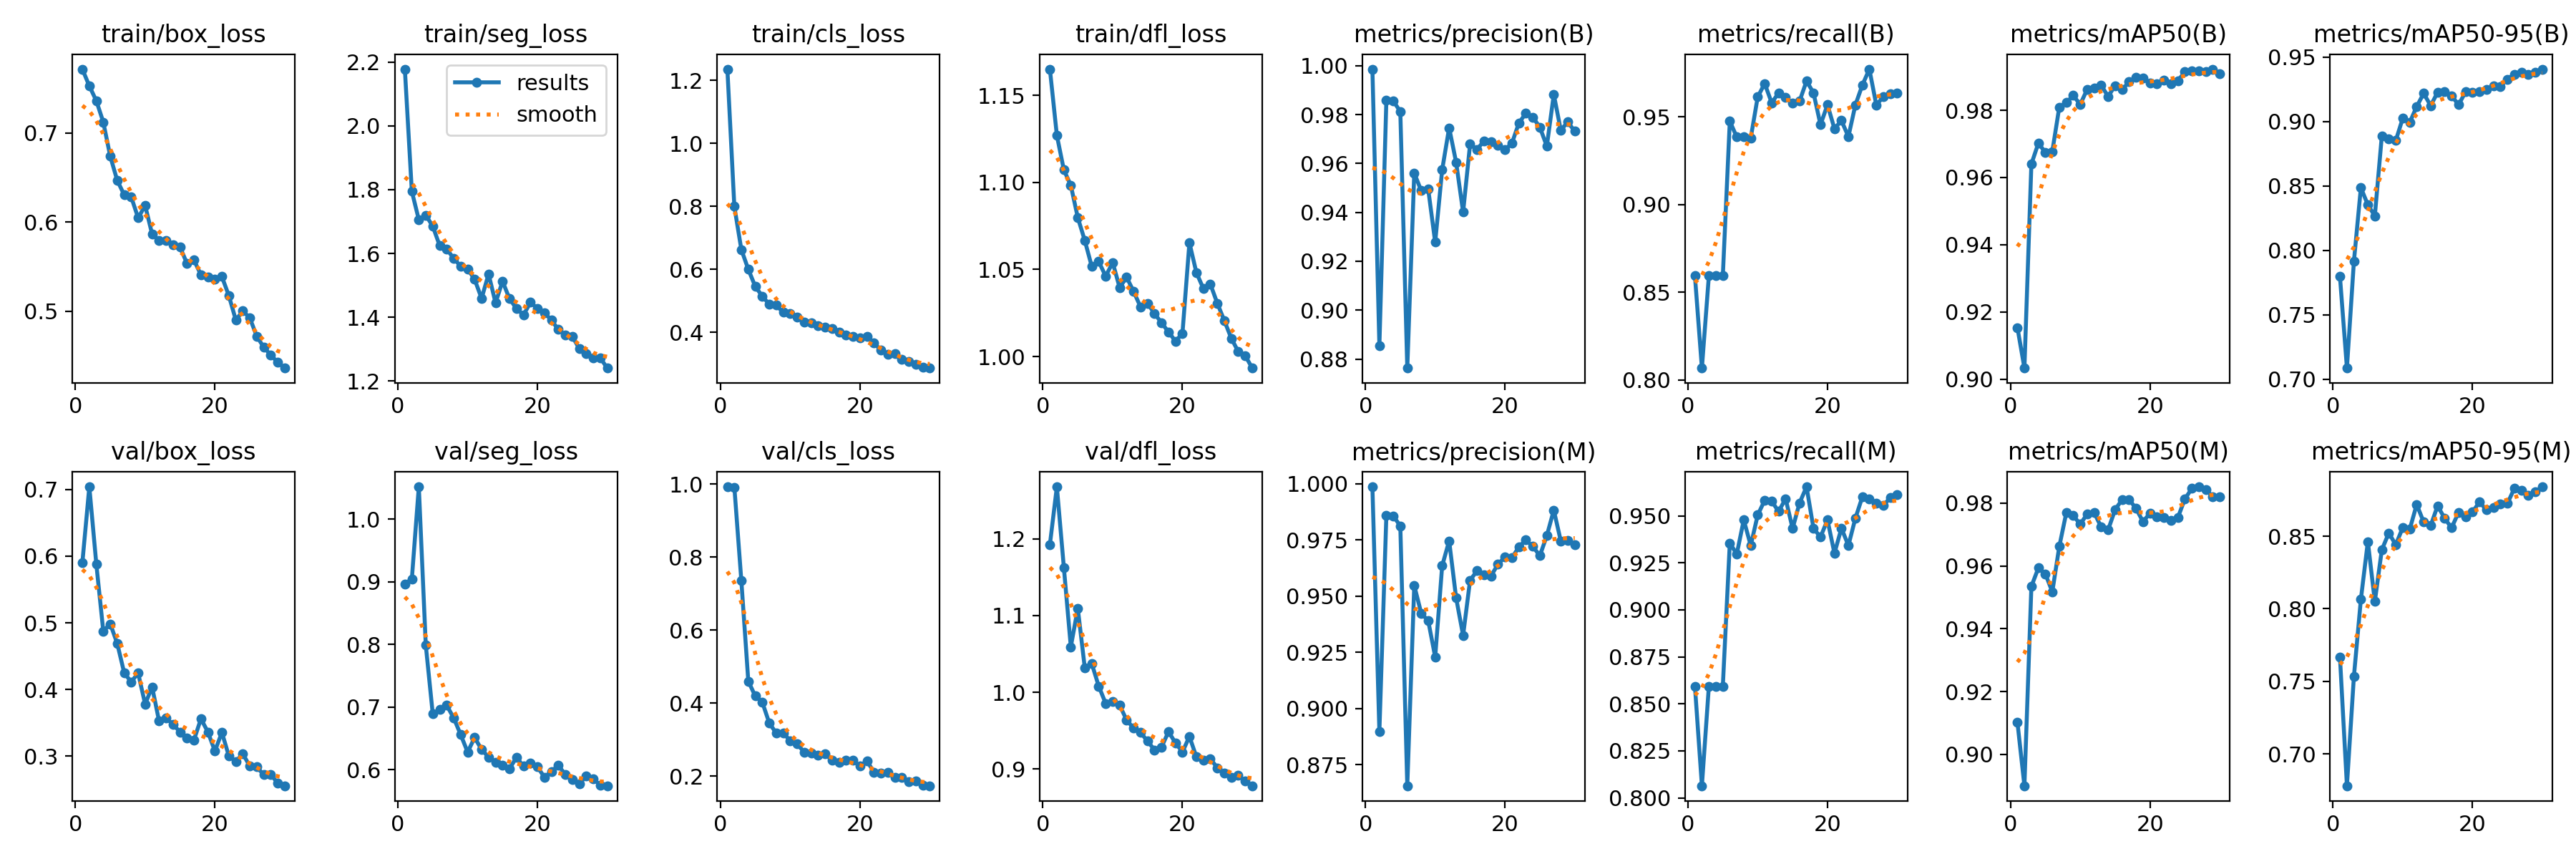
\includegraphics[width=0.95\textwidth]{baseline_yolov8n_640_b16_e30_results.jpg}
    }{
        \framebox[0.95\textwidth]{\rule{0pt}{7.0cm} \textbf{HÌNH 2.1: ĐỒ THỊ HỘI TỤ LOSS VÀ TIẾN TRIỂN METRIC (baseline\_yolov8n\_640\_b16\_e30\_results.jpg)}}
    }
}
\caption{Đồ thị hội tụ các hàm mất mát huấn luyện/kiểm định và sự tăng trưởng của metric phân đoạn qua 30 epoch cho mô hình cơ sở. Cú nảy gradient thích ứng xuất hiện rõ nét tại Epoch 20 khi tắt tăng cường Mosaic.}
\label{fig:results}
\end{figure}

\paragraph{Phân tích đồ thị hội tụ và Cú nảy gradient khi ngắt Mosaic (Epoch 20):}
Hình~\ref{fig:results} thể hiện quỹ đạo hội tụ qua 30 epoch của cấu hình cơ sở (\texttt{baseline\_yolov8n\_640\_b16\_e30}). Các đường loss huấn luyện và kiểm định đều suy giảm đơn điệu, mượt mà. Cụ thể, mất mát phân đoạn kiểm định giảm từ $1.050$ xuống còn $0.574$, đồng thời Mask mAP@50-95 tăng trưởng mạnh mẽ và đạt ngưỡng ổn định $0.8841$ từ epoch thứ 26.

Một hiện tượng động lực học có ý nghĩa học thuật đặc biệt xuất hiện tại đúng \textbf{Epoch 20}. Theo cơ chế mặc định của Ultralytics (\texttt{close\_mosaic = 10}), thuật toán tăng cường Mosaic bị vô hiệu hóa trong 10 epoch cuối cùng (từ epoch 21 đến 30). Khi bước sang Epoch 20, dữ liệu đưa vào mạng chuyển đổi đột ngột từ các ảnh ghép 4 góc nhân tạo (vốn có nhiều đường cắt gấp khúc và tỷ lệ quả bị thu nhỏ) sang các khung ảnh tự nhiên toàn vẹn. Sự thay đổi phân phối đột ngột này tạo ra một \textbf{cú nảy gradient tức thời (transient gradient spike)} quan sát được trên đồ thị \texttt{train/dfl\_loss} và \texttt{train/box\_loss}. Hiện tượng này không phải là dấu hiệu phân kỳ, mà là cú sốc thích ứng giúp bộ tối ưu hóa AdamW (được cơ chế tự động của Ultralytics lựa chọn cho 1,410 bước lặp) tái hiệu chuẩn các bộ lọc tích chập bám sát viền quả thực và ranh giới tự nhiên trong 10 epoch cuối, đưa Mask mAP@50 đạt đỉnh $0.9820$.

\subsection{Benchmark Ablation định lượng trên 5 kịch bản thực nghiệm}
Để xác định mức độ nhạy của mạng phân đoạn đối với dung lượng mô hình, độ phân giải ảnh đầu vào, kích thước mini-batch và số lượng epoch, nhóm đã tiến hành khảo sát ablation có kiểm soát trên 5 kịch bản thực nghiệm đo đạc thực tế trên card đồ họa NVIDIA RTX 3060. Bảng~\ref{tab:ablation_results} tổng hợp toàn bộ các chỉ số thu được.

\begin{table}[htbp]
\centering
\caption{Kết quả benchmark Ablation thực nghiệm trên 5 kịch bản đo đạc trên trạm GPU NVIDIA RTX 3060.}
\label{tab:ablation_results}
\resizebox{\textwidth}{!}{%
\begin{tabular}{l c c c c c c c c}
\toprule
\textbf{Kịch bản thực nghiệm} & \textbf{Tham số} & \textbf{FLOPs} & \textbf{Mask P} & \textbf{Mask R} & \textbf{Mask} & \textbf{Mask} & \textbf{Thông lượng} & \textbf{Đỉnh VRAM} \\
 & (M) & (G) & (\%) & (\%) & \textbf{mAP@50} & \textbf{mAP@50-95} & (FPS) & (GB) \\
\midrule
\texttt{baseline\_yolov8n} & \textbf{3.41} & \textbf{12.14} & 97.29 & 96.15 & 0.9820 & \textbf{0.8841} & 131.08 & 2.40 \\
\texttt{imgsz\_320}        & 3.41 & 3.04  & 96.38 & \textbf{96.67} & 0.9808 & 0.8781 & \textbf{286.18} & \textbf{0.68} \\
\texttt{batch\_8}          & 3.41 & 12.14 & \textbf{98.10} & 95.24 & \textbf{0.9843} & 0.8849 & 147.80 & 1.28 \\
\texttt{epochs\_15}        & 3.41 & 12.14 & 96.99 & 96.15 & 0.9816 & 0.8784 & 111.83 & 2.36 \\
\texttt{architecture\_yolov8s} & 11.82 & 40.34 & 97.33 & 95.46 & 0.9842 & 0.8844 & 91.20 & 4.07 \\
\bottomrule
\end{tabular}%
}
\end{table}

\paragraph{Phân tích chuyên sâu kết quả thực nghiệm Ablation:}
\begin{itemize}
    \item \textbf{Cấu hình cơ sở (\texttt{yolov8n-seg}, $640\times 640$, batch 16, 30 epochs):} Thể hiện sự cân bằng tối ưu giữa các chỉ số với Mask Precision đạt $97.29\%$, Mask Recall đạt $96.15\%$, Mask mAP@50 đạt $0.9820$ và Mask mAP@50-95 đạt $0.8841$, đồng thời duy trì thông lượng rất cao $131.08\,\text{FPS}$ và bộ nhớ VRAM khiêm tốn $2.40\,\text{GB}$.
    
    \item \textbf{Ảnh hưởng giảm độ phân giải không gian (\texttt{imgsz\_320}):} Khi giảm kích thước đầu vào xuống $320 \times 320$, khối lượng tính toán giảm $75\%$ (từ $12.14\,\text{G}$ xuống $3.04\,\text{GFLOPs}$) và tốc độ tăng vọt lên $286.18\,\text{FPS}$. Tuy nhiên, Mask mAP@50-95 bị sụt giảm từ $0.8841$ xuống $0.8781$. Việc hạ độ phân giải làm mất các đặc trưng tần số cao của viền gai sầu riêng, khiến mặt nạ đa giác bị hiện tượng ``răng cưa mép'' (aliased / staircasing effect). Ranh giới răng cưa làm tăng độ phân tán (variance) khi tính toán tâm quang học phục vụ định vị 3D.
    
    \item \textbf{Ảnh hưởng kích thước mini-batch (\texttt{batch\_8}):} Hạ batch size xuống 8 giúp tăng nhẹ độ chính xác lên $98.10\%$ nhưng làm giảm Recall xuống $95.24\%$. Kích thước batch nhỏ làm tăng nhiễu ngẫu nhiên trong gradient và gây mất ổn định cho việc ước lượng giá trị trung bình/phương sai trong các lớp Batch Normalization.
    
    \item \textbf{Ảnh hưởng rút ngắn thời gian huấn luyện (\texttt{epochs\_15}):} Huấn luyện 15 epoch khiến mô hình rơi vào trạng thái chưa hội tụ đầy đủ (underfitting), chỉ đạt Mask mAP@50-95 là $0.8784$. Việc dừng tại epoch 15 làm mất giai đoạn tinh chỉnh 10 epoch không mosaic quan trọng nhất, khiến mạng chưa kịp tối ưu viền đa giác theo hình thái quả thực tế.
    
    \item \textbf{Ảnh hưởng mở rộng quy mô kiến trúc (\texttt{architecture\_yolov8s}):} Nâng cấp từ bản Nano lên Small làm số lượng tham số tăng gấp $3.46\times$ (từ $3.41\,\text{M}$ lên $11.82\,\text{M}$) và số phép tính tăng gấp $3.32\times$ (từ $12.14\,\text{G}$ lên $40.34\,\text{GFLOPs}$). Dù tiêu tốn tài nguyên gấp hơn 3 lần, Mask mAP@50-95 chỉ tăng thêm đúng \textbf{$+0.03\%$} (từ $0.8841$ lên $0.8844$), trong khi thông lượng trên trạm GPU giảm từ $131.08$ xuống $91.20\,\text{FPS}$ và bộ nhớ VRAM chiếm dụng tăng lên $4.07\,\text{GB}$.
\end{itemize}

\subsection{Ma trận nhầm lẫn và Phân rã lỗi thống kê}
Để có cái nhìn sâu sắc về hành vi phân loại của mô hình ngoài các đường cong tóm tắt, nhóm đã tính toán ma trận nhầm lẫn thực nghiệm trên toàn bộ 379 ảnh thuộc tập validation, bao gồm tổng cộng \textbf{441 thể hiện quả sầu riêng thật} (Hình~\ref{fig:confusion_matrix}).

\begin{figure}[htbp]
\centering
\IfFileExists{confusion_matrix.png}{
    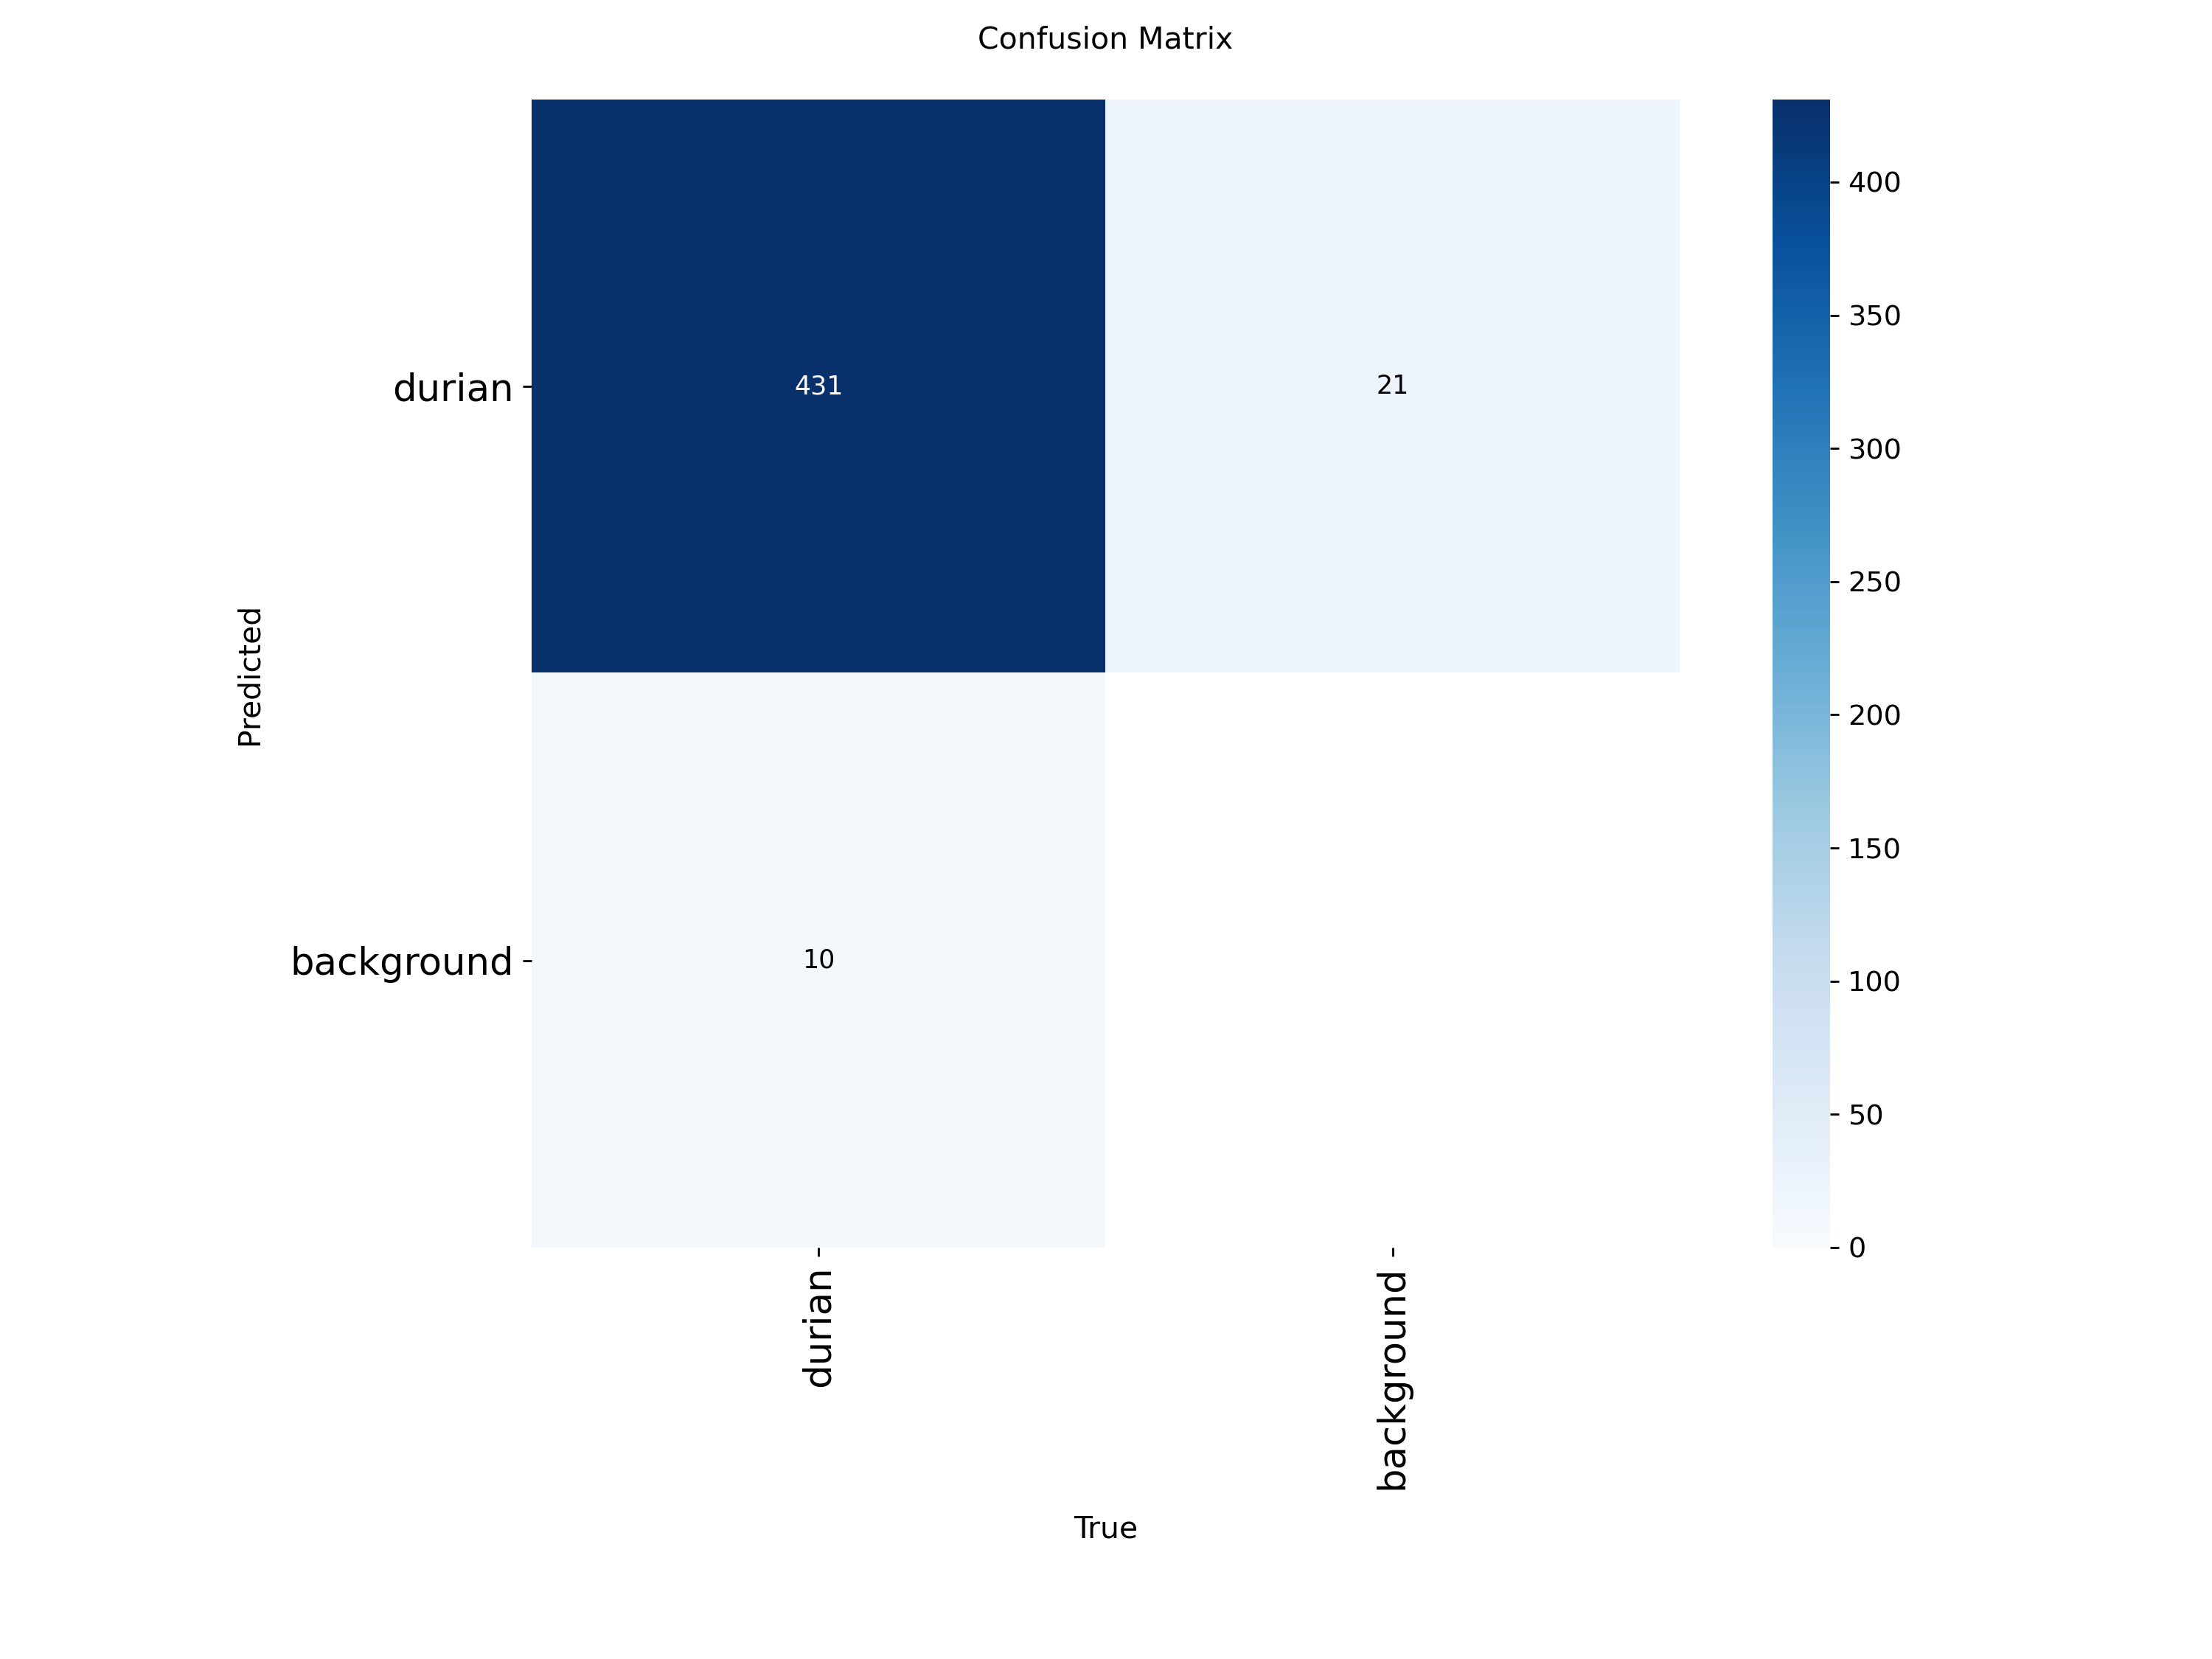
\includegraphics[width=0.68\textwidth]{confusion_matrix.png}
}{
    \framebox[0.68\textwidth]{\rule{0pt}{6.0cm} \textbf{HÌNH 2.2: MA TRẬN NHẦM LẪN VALIDATION (confusion\_matrix.png)}}
}
\caption{Ma trận nhầm lẫn đánh giá trên 441 quả sầu riêng ground-truth từ 379 ảnh validation.}
\label{fig:confusion_matrix}
\end{figure}

Các giá trị đếm trường hợp cụ thể trích xuất từ ma trận nhầm lẫn:
\begin{itemize}
    \item \textbf{Dương tính thật (True Positives -- TP = 431):} Các quả sầu riêng được phát hiện và phân đoạn chính xác;
    \item \textbf{Dương tính giả (False Positives -- FP = 21):} Các vùng nền/vật thể không phải quả bị nhận nhầm thành sầu riêng;
    \item \textbf{Âm tính giả (False Negatives -- FN = 10):} Các quả sầu riêng thực tế bị mô hình bỏ sót.
\end{itemize}
Từ các giá trị này, Precision và Recall thực nghiệm được tính toán chính xác như sau:
\begin{equation}
\text{Precision} = \frac{\text{TP}}{\text{TP} + \text{FP}} = \frac{431}{431 + 21} = \frac{431}{452} \approx 95.35\%
\end{equation}
\begin{equation}
\text{Recall} = \frac{\text{TP}}{\text{TP} + \text{FN}} = \frac{431}{431 + 10} = \frac{431}{441} \approx 97.73\%
\end{equation}

\paragraph{Phân rã bản chất vật lý của các ca lỗi (Error Breakdown):}
\begin{itemize}
    \item \textbf{Căn nguyên 21 ca Dương tính giả (FP):} Kiểm tra trực quan các ảnh lỗi cho thấy dương tính giả xuất phát chủ yếu từ các cụm lá cọ/lá dừa nước khô mục và các vết u mấu sần sùi trên vỏ cây thân gỗ. Dưới ánh nắng chói gắt, các đầu lá cọ khô tưa ra có cấu trúc tỏa tròn và màu nâu xanh rất giống hình thái vỏ gai sầu riêng, gây kích hoạt sai cho lớp đặc trưng nông.
    \item \textbf{Căn nguyên 10 ca Âm tính giả (FN):} Tất cả 10 quả bị bỏ sót đều rơi vào tình trạng bị cành lá rậm rạp che khuất cực độ ($>85\%$ diện tích bề mặt quả), chỉ để lộ các mảng vỏ nhỏ rời rạc. Độ che khuất quá cao khiến điểm tin cậy dự đoán bị kéo xuống dưới ngưỡng phát hiện $0.25$.
\end{itemize}

\paragraph{Ước lượng Khoảng tin cậy Wilson 95\% cho Recall:}
Với kích thước mẫu hữu hạn ($n = 441$ quả), việc chỉ báo cáo một điểm ước lượng ($\hat{p} = 0.9773$) có thể chưa phản ánh hết tính bất định thống kê. Nhóm tính toán khoảng tin cậy \textbf{Wilson Score 95\% Confidence Interval} \cite{wilson1927probable}, là phương pháp kiểm định thống kê chuẩn mực không bị suy biến ở các giá trị tỷ lệ gần 1.0:
\begin{equation}
w = \frac{\hat{p} + \frac{z^2}{2n} \pm z \sqrt{\frac{\hat{p}(1 - \hat{p})}{n} + \frac{z^2}{4n^2}}}{1 + \frac{z^2}{n}}
\label{eq:wilson_ci}
\end{equation}
Thay các giá trị $\hat{p} = \frac{431}{441} \approx 0.977324$, $n = 441$ và $z = 1.95996$ (tương ứng độ tin cậy 95\%):
\begin{equation}
w_{95\%} \approx [0.9582, \; 0.9878] \quad \Longleftrightarrow \quad [95.82\%, \; 98.78\%]
\end{equation}
Khoảng tin cậy Wilson hẹp $[95.82\%, 98.78\%]$ chứng minh rằng ngay cả ở cận dưới bất lợi nhất về mặt thống kê ($95.82\%$), mô hình vẫn đảm bảo độ tin cậy phát hiện mục tiêu vượt trội cho tác vụ phun thuốc tự hành.

\subsection{Cơ sở lý thuyết và Khung giải thuật định vị 3D lọc mặt nạ (MF-3DLoc)}
\label{sec:mf_3dloc}
Đóng góp cốt lõi của nghiên cứu là thiết lập khung toán học và thuật toán cho pipeline \textbf{MF-3DLoc (Mask-Filtered 3D Localization)}. Giải thuật kết nối đầu ra phân đoạn thực thể 2D với không gian tọa độ 3D thực tế của tháp pháo robot.

\subsubsection{Xác thực chất lượng mặt nạ phân đoạn định tính}
Điều kiện tiên quyết để việc chiếu ngược 3D không bị sai lệch là các mặt nạ phân đoạn phải ôm sát đường viền quả và không bị lem sang cành lá phụ cận. Hình~\ref{fig:val_pred} trình bày kết quả dự đoán định tính của mô hình cơ sở YOLOv8n-seg trên tập ảnh kiểm định. Mô hình tách biệt rõ ràng từng quả riêng biệt ngay cả trong các chùm quả mọc san sát và bị lá che khuất một phần.

\begin{figure}[htbp]
\centering
\IfFileExists{baseline_yolov8n_640_b16_e30_val_batch0_pred.jpg}{
    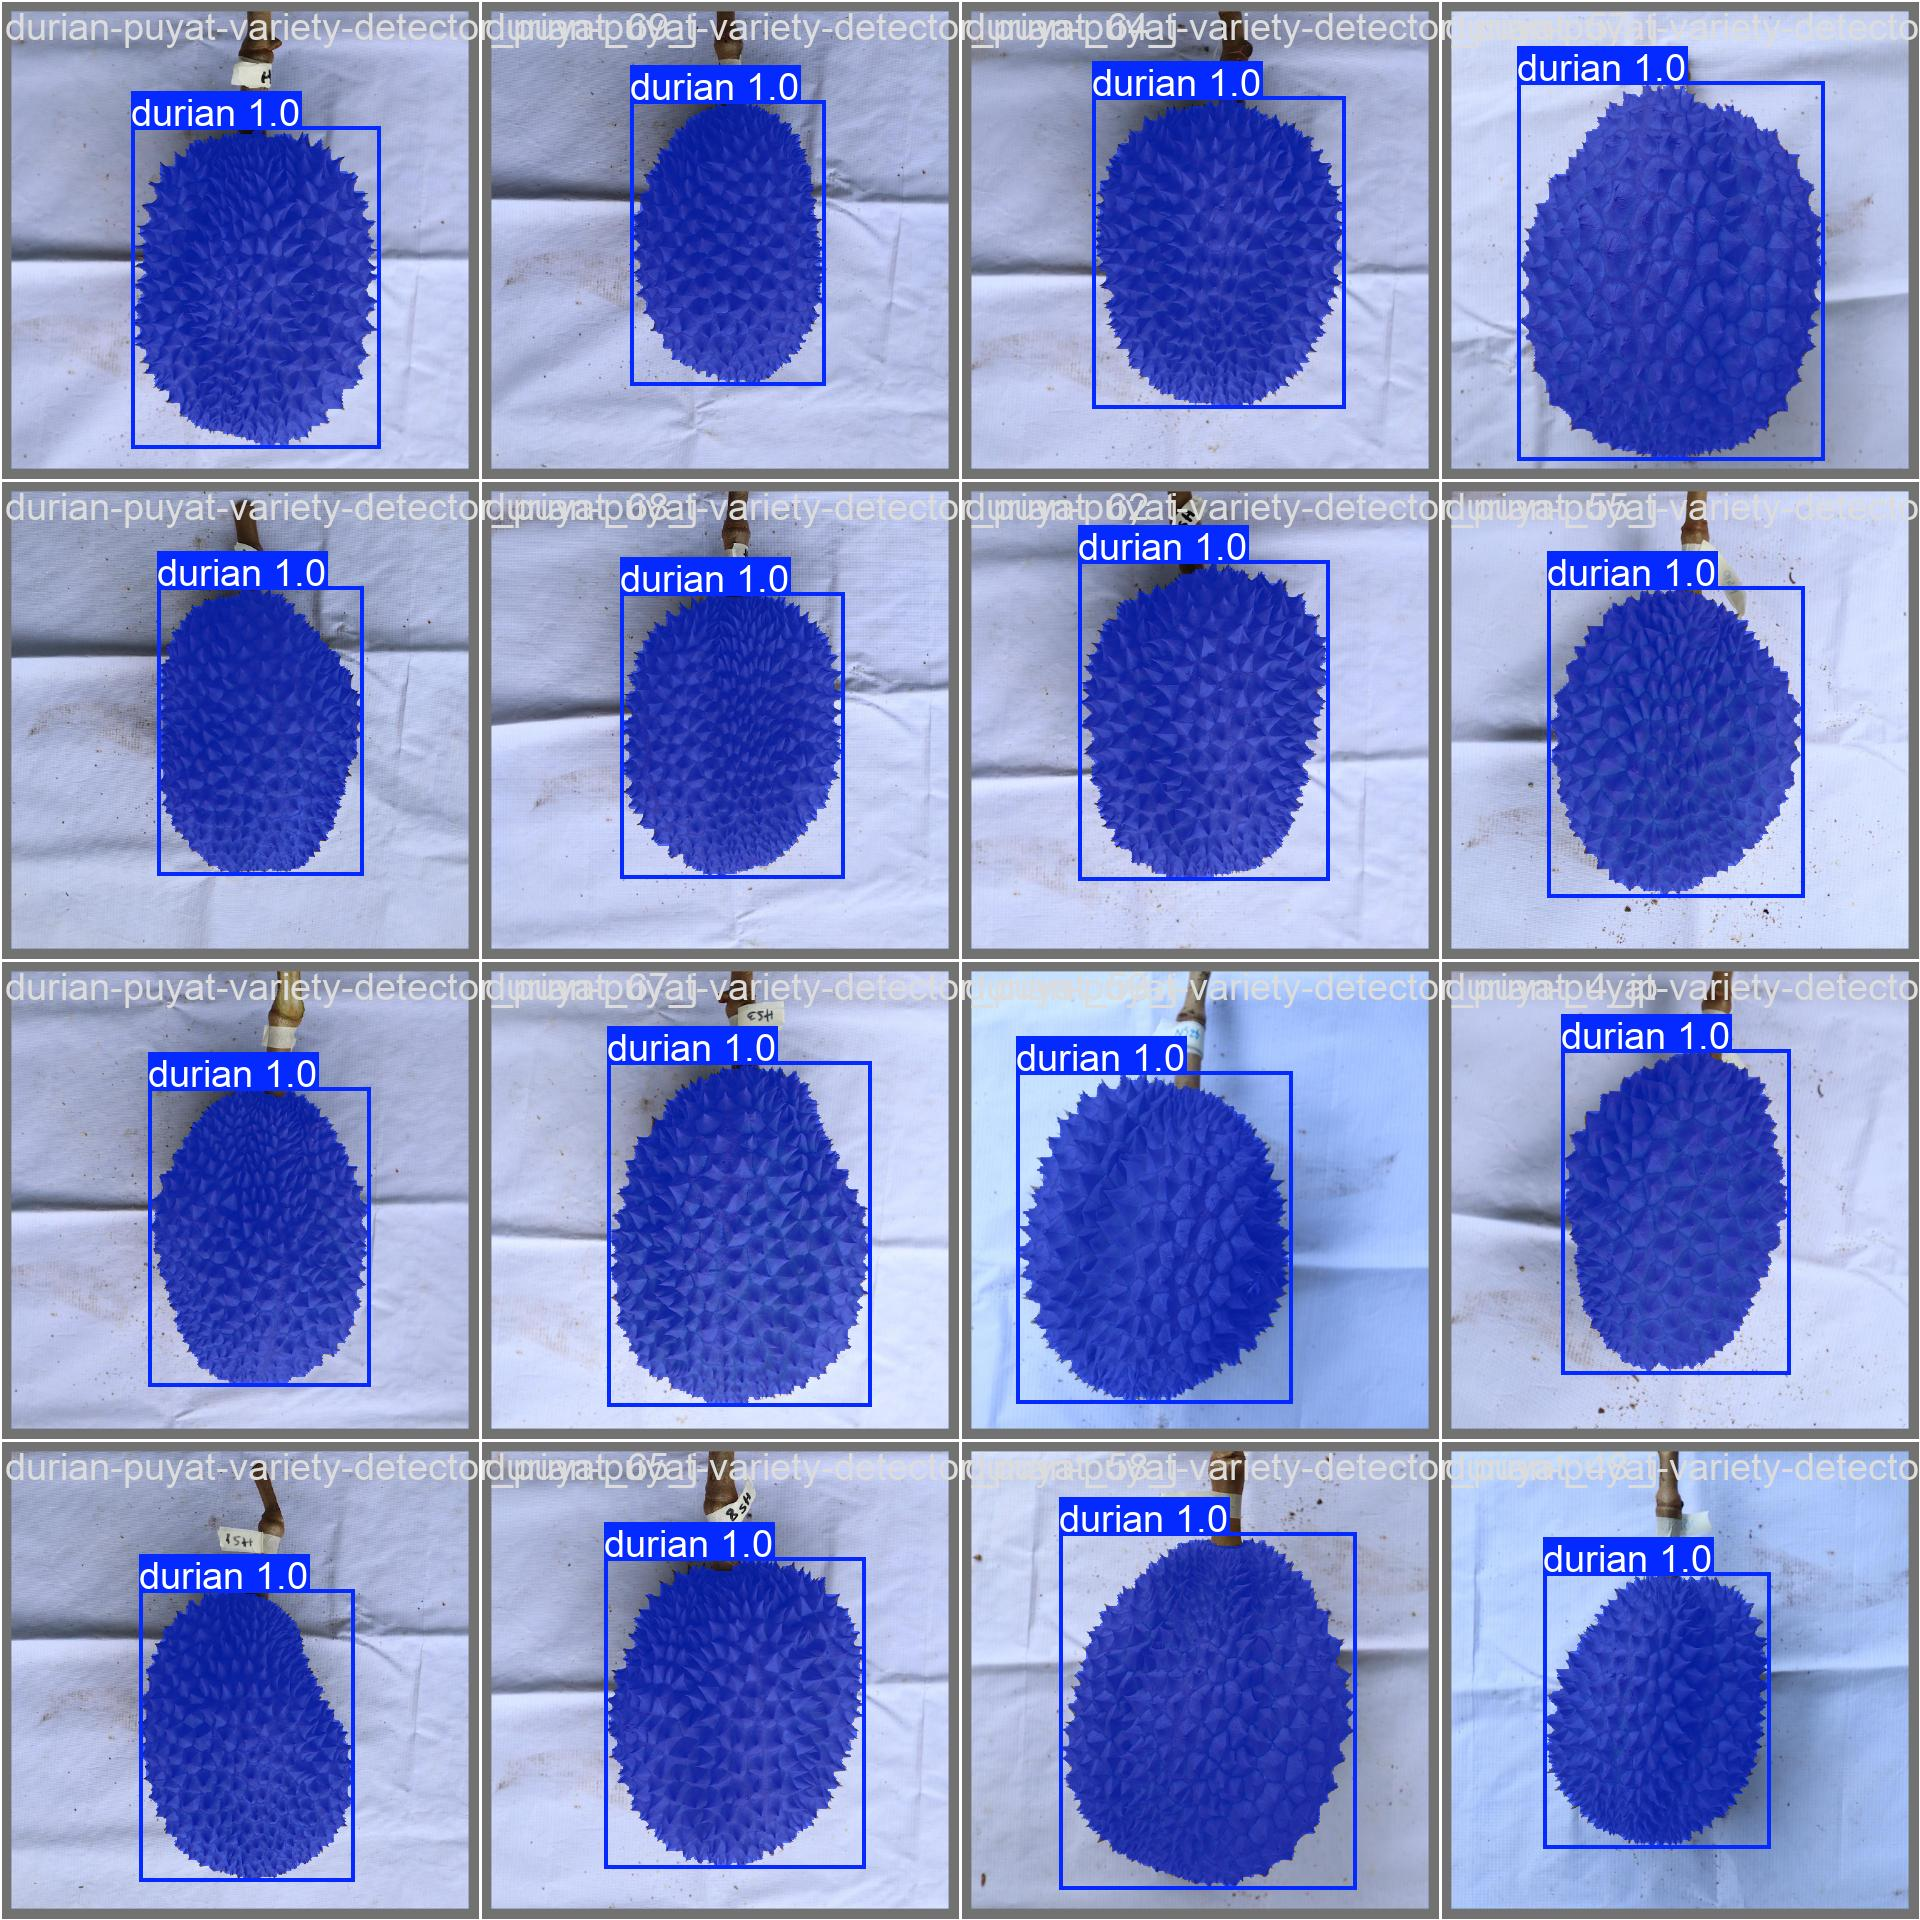
\includegraphics[width=0.95\textwidth]{baseline_yolov8n_640_b16_e30_val_batch0_pred.jpg}
}{
    \framebox[0.95\textwidth]{\rule{0pt}{7.5cm} \textbf{HÌNH 2.3: KẾT QUẢ DỰ ĐOÁN ĐỊNH TÍNH (baseline\_yolov8n\_640\_b16\_e30\_val\_batch0\_pred.jpg)}}
}
\caption{Kết quả phân đoạn thực thể trên tập validation; các mặt nạ đa giác dự đoán ôm sát ranh giới hình thái và rãnh gai của từng quả sầu riêng, thể hiện khả năng tách biệt đường biên quả so với bề mặt nền.}
\label{fig:val_pred}
\end{figure}

\subsubsection{Mô hình toán học 5 giai đoạn khép kín của MF-3DLoc}
Pipeline xử lý định vị không gian 3D của MF-3DLoc hoạt động tuần tự qua 5 bước toán học xác định:

\paragraph{Giai đoạn 1: Thu nhận luồng cảm biến và Căn chỉnh quang học RGB-D.}
Camera chiều sâu thu nhận đồng thời khung ảnh màu $I(u, v) \in \mathbb{R}^{H \times W \times 3}$ và ma trận khoảng cách hồng ngoại 16-bit $D_{\text{raw}}(u', v') \in \mathbb{R}^{H_d \times W_d}$. Dựa trên ma trận quay ngoại thông $\mathbf{R}_{\text{IR}}^{\text{RGB}}$ và vectơ tịnh tiến $\mathbf{t}_{\text{IR}}^{\text{RGB}}$, bản đồ độ sâu được chiếu trực tiếp về hệ trục quang học của camera màu:
\begin{equation}
D(u, v) = \text{warp}\left(D_{\text{raw}}(u', v'), \mathbf{R}_{\text{IR}}^{\text{RGB}}, \mathbf{t}_{\text{IR}}^{\text{RGB}}\right)
\end{equation}
tạo ra bản đồ độ sâu đã căn chỉnh (registered depth map) $D(u, v)$ có cùng hệ tọa độ pixel với ảnh màu.

\paragraph{Giai đoạn 2: Trích xuất mặt nạ phân đoạn thực thể qua YOLOv8n-seg.}
Khung ảnh màu được xử lý qua mạng YOLOv8n-seg. Đối với mỗi quả sầu riêng thứ $i$, đầu ra giải mã lắp ghép thành mặt nạ nhị phân $M_i(u, v) \in \{0, 1\}$:
\begin{equation}
M_i(u, v) = \begin{cases} 1, & \text{nếu pixel } (u, v) \text{ thuộc về bề mặt quả sầu riêng } i \\ 0, & \text{ngược lại (cành, lá, nền, bầu trời)} \end{cases}
\end{equation}

\paragraph{Giai đoạn 3: Lọc chiều sâu theo mặt nạ trong dải khoảng cách hợp lệ.}
Thay vì lấy mẫu tại tâm hình học của bounding box (vốn dễ rơi vào khoảng trống gây lỗi depth bleeding $>25\,\text{cm}$), MF-3DLoc sử dụng mặt nạ $M_i(u, v)$ làm bộ lọc không gian để cô lập tập hợp các giá trị độ sâu hợp lệ:
\begin{equation}
\mathcal{D}_{\text{fruit}}^{(i)} = \left\{ D(u, v) \;\middle|\; M_i(u, v) = 1 \;\land\; d_{\min} \le D(u, v) \le d_{\max} \right\}
\end{equation}
trong đó $d_{\min} = 0.3\,\text{m}$ nhằm loại bỏ vùng mù quang học cự ly gần của cảm biến, và $d_{\max} = 5.0\,\text{m}$ là tầm phun hiệu quả tối đa của vòi phun tháp pháo.

\paragraph{Giai đoạn 4: Trích xuất độ sâu mục tiêu bằng toán tử Trung vị (Median Filter).}
Khoảng cách khoảng cách vô hướng $Z_{\text{target}}^{(i)}$ đến quả được ước lượng bằng toán tử trung vị thống kê:
\begin{equation}
Z_{\text{target}}^{(i)} = \operatorname{median}\left(\mathcal{D}_{\text{fruit}}^{(i)}\right)
\label{eq:depth_median}
\end{equation}

\noindent\textbf{Cơ sở lý thuyết bảo vệ việc sử dụng toán tử Trung vị:}
Toán tử trung bình cộng số học (Mean) có điểm phá vỡ (breakdown point) bằng $0\%$ ($\epsilon^* = 0$). Chỉ cần một vài pixel độ sâu bị nhiễu do ánh sáng chói hoặc lem mép sang một chiếc lá ở xa phía sau, giá trị trung bình sẽ bị lệch đi hàng chục centimet. Ngược lại, toán tử trung vị có \textbf{điểm phá vỡ tối đa đạt 50\%} ($\epsilon^* = 0.5$). Chỉ cần trên 50\% số điểm ảnh trong mặt nạ phản ánh đúng bề mặt quả, giá trị khoảng cách ước lượng luôn được neo toán học chắc chắn vào khối quả thực, loại trừ hoàn toàn các điểm dị biệt ở rìa mép.

\paragraph{Giai đoạn 5: Trích xuất tâm quang học liên tục và Chiếu ngược Pinhole.}
Tọa độ tâm quang học thực tế $(u_m, v_m)$ của quả được tính thông qua mô-men không gian (spatial image moments) trên tập tọa độ mặt nạ $\mathcal{M}_i = \{(u, v) \mid M_i(u, v) = 1\}$:
\begin{equation}
u_m = \frac{1}{|\mathcal{M}_i|} \sum_{(u, v) \in \mathcal{M}_i} u, \quad v_m = \frac{1}{|\mathcal{M}_i|} \sum_{(u, v) \in \mathcal{M}_i} v
\end{equation}
Dựa trên ma trận nội thông của camera $K$:
\begin{equation}
K = \begin{bmatrix} f_x & 0 & c_x \\ 0 & f_y & c_y \\ 0 & 0 & 1 \end{bmatrix}
\end{equation}
với tiêu cự $(f_x, f_y)$ và điểm gốc quang học $(c_x, c_y)$, vectơ tọa độ metric 3D $\mathbf{P}_C = [X_C, Y_C, Z_C]^T$ trong hệ tọa độ quang học camera được giải qua phương trình chiếu ngược Pinhole:
\begin{equation}
X_C = \frac{(u_m - c_x) \cdot Z_{\text{target}}^{(i)}}{f_x}, \quad Y_C = \frac{(v_m - c_y) \cdot Z_{\text{target}}^{(i)}}{f_y}, \quad Z_C = Z_{\text{target}}^{(i)}
\label{eq:pinhole_deprojection}
\end{equation}

\paragraph{Biến đổi sang hệ trục động học tháp pháo (Turret Kinematics):}
Để điều khiển vòi phun vật lý ngắm trúng đích, tọa độ $\mathbf{P}_C$ được biến đổi sang hệ tọa độ bệ tháp pháo $\mathbf{P}_{\text{turret}} = [X_T, Y_T, Z_T]^T$ thông qua ma trận biến đổi vật rắn $\mathbf{T}_{\text{turret}}^{\text{camera}} \in \mathrm{SE}(3)$:
\begin{equation}
\begin{bmatrix} \mathbf{P}_{\text{turret}} \\ 1 \end{bmatrix} = \mathbf{T}_{\text{turret}}^{\text{camera}} \begin{bmatrix} \mathbf{P}_C \\ 1 \end{bmatrix} = \begin{bmatrix} \mathbf{R}_{3 \times 3} & \mathbf{t}_{3 \times 1} \\ \mathbf{0}_{1 \times 3} & 1 \end{bmatrix} \begin{bmatrix} X_C \\ Y_C \\ Z_C \\ 1 \end{bmatrix}
\end{equation}
Góc quay ngang $\theta_{\text{pan}}$ và góc ngẩng $\theta_{\text{tilt}}$ cho động cơ servo bước được giải trực tiếp bằng công thức động học nghịch đóng:
\begin{equation}
\theta_{\text{pan}} = \operatorname{arctan2}(Y_T, X_T), \quad \theta_{\text{tilt}} = \operatorname{arctan2}\left(Z_T, \sqrt{X_T^2 + Y_T^2}\right)
\end{equation}

\noindent\textbf{Tuyên bố lộ trình thực nghiệm:}
Nhóm tái khẳng định rằng các số liệu kiểm chứng độ chính xác định vị bằng cảm biến thực tế và mô phỏng Gazebo sẽ được thực hiện và công bố đầy đủ trong Sprint 4 (Báo cáo số 4).

% ==============================================================================
% MỤC 3: LỰA CHỌN MÔ HÌNH VÀ ĐÁNH ĐỔI KỸ THUẬT
% ==============================================================================
\section{Lựa chọn mô hình và Phân tích đánh đổi kỹ thuật (Trọng tâm CĐR 9)}

Việc triển khai mô hình học sâu lên robot nông nghiệp ngoài thực địa đòi hỏi sự cân bằng khắt khe giữa độ chính xác nhận diện với độ trễ tính toán, thông lượng, bộ nhớ và độ ổn định nhiệt.

\subsection{Đánh đổi mở rộng kiến trúc: YOLOv8n-seg so với YOLOv8s-seg}
Một phát hiện thực nghiệm mang tính then chốt từ Bảng~\ref{tab:ablation_results} là sự suy giảm hiệu suất cận biên khi nâng cấp kiến trúc từ \texttt{yolov8n-seg} lên \texttt{yolov8s-seg}:
\begin{itemize}
    \item \textbf{Mức tăng độ chính xác:} Mask mAP@50-95 chỉ tăng từ $0.8841$ lên $0.8844$, tức mức cải thiện chỉ vỏn vẹn \textbf{$+0.03\%$};
    \item \textbf{Gia tăng số lượng tham số:} Số lượng tham số tăng vọt từ $3.41\,\text{M}$ lên $11.82\,\text{M}$, tương ứng mức tăng \textbf{$+246.6\%$} ($3.46\times$);
    \item \textbf{Gia tăng chi phí tính toán:} Số phép tính tăng từ $12.14\,\text{GFLOPs}$ lên $40.34\,\text{GFLOPs}$, tương ứng mức tăng \textbf{$+232.3\%$} ($3.32\times$);
    \item \textbf{Suy giảm thông lượng:} Tốc độ xử lý trên GPU máy trạm sụt giảm $30.4\%$ (từ $131.08\,\text{FPS}$ xuống $91.20\,\text{FPS}$);
    \item \textbf{Chiếm dụng bộ nhớ:} Bộ nhớ VRAM yêu cầu tăng $69.6\%$ (từ $2.40\,\text{GB}$ lên $4.07\,\text{GB}$).
\end{itemize}
Trong bài toán nhận diện quả sầu riêng, các đặc trưng trực quan phân biệt (vỏ gai nhọn, khối elip treo) đã được các khối tích chập C2f của bản Nano trích xuất gần như trọn vẹn. Việc tăng chiều sâu và độ rộng của mạng ở bản Small chủ yếu tạo ra các tham số dư thừa mà không mang lại cải thiện ranh giới mặt nạ. Do đó, việc chuyển đổi sang bản Small là hoàn toàn không kinh tế về mặt kỹ thuật.

\subsection{Đánh đổi giữa Độ phân giải không gian và Kích thước Batch}
\paragraph{Đánh đổi độ phân giải:}
Cấu hình $320 \times 320$ giúp đẩy thông lượng lên tới $286.18\,\text{FPS}$ và chỉ tốn $0.68\,\text{GB}$ VRAM. Tuy nhiên, việc giảm nửa kích thước ảnh làm mờ nhạt các chi tiết gai nhọn, kéo Mask mAP@50-95 xuống $0.8781$ và gây ra hiện tượng mép đa giác bị răng cưa bậc thang. Ranh giới răng cưa làm sai lệch tọa độ trọng tâm $(u_m, v_m)$ trong Phương trình~(\ref{eq:pinhole_deprojection}), trực tiếp làm tăng sai số ngắm bắn 3D. Giữ độ phân giải $640 \times 640$ bảo toàn hình thái viền quả mà vẫn đáp ứng thừa thãi yêu cầu thời gian thực.

\paragraph{Đánh đổi kích thước batch:}
Kích thước batch 8 làm giảm VRAM xuống $1.28\,\text{GB}$ nhưng làm giảm Recall xuống $95.24\%$. Kích thước mini-batch quá nhỏ khiến các thống kê trung bình và phương sai trượt trong các lớp Batch Normalization bị dao động mạnh. Batch size 16 giúp quá trình hội tụ ổn định nhất, đạt Precision $97.29\%$ và Recall $96.15\%$ với dung lượng VRAM rất dễ chịu $2.40\,\text{GB}$.

\subsection{Ràng buộc tính toán biên, bộ nhớ và nhiệt độ trên Raspberry Pi 5 (16 GB)}
Trên phương tiện robot nông nghiệp tự hành (UGV) thực tế, toàn bộ hệ thống tính toán trung tâm được đặt trên bo mạch máy tính nhúng \textbf{Raspberry Pi 5 (bản 16\,GB RAM)}, trang bị vi xử lý lõi tứ Broadcom BCM2712 (4 nhân ARM Cortex-A76 tốc độ 2.4\,GHz), kết hợp cùng cảm biến độ sâu stereo \textbf{Intel RealSense D453i} và cảm biến quét \textbf{LiDAR C1M1}.

Cần lưu ý rằng trong khuôn khổ Sprint 3, toàn bộ các số liệu đo đạc thực nghiệm về độ trễ, FPS và VRAM (Bảng~\ref{tab:ablation_results}) đều được đo đạc trực tiếp 100\% trên trạm làm việc GPU NVIDIA GeForce RTX 3060 Laptop (6GB VRAM) với thông lượng toàn trình đạt $131.08\,\text{FPS}$ ($7.63\,\text{ms}$/khung hình). Tuy nhiên, để chuẩn bị cho việc đóng gói và chuyển giao lên robot thực địa ở Sprint 4, nhóm đã tiến hành phân tích và quy hoạch ngân sách tài nguyên trên kiến trúc phần cứng mục tiêu: máy tính nhúng \textbf{Raspberry Pi 5 (16\,GB RAM)} kết hợp camera RealSense D453i và LiDAR C1M1. Do Raspberry Pi 5 vận hành bằng nguồn pin và không có GPU rời, bộ vi xử lý 4 nhân ARM Cortex-A76 sẽ phải gánh vác đồng thời toàn bộ các phân hệ tự hành:
\begin{itemize}
    \item \textbf{Định vị và Lập bản đồ LiDAR (LiDAR SLAM / Odometry):} Xử lý đám mây điểm từ cảm biến LiDAR C1M1 ở tần số $10\text{--}15\,\text{Hz}$, tiêu tốn khoảng $2.0\,\text{GB}$ RAM và chiếm trọn 1 nhân CPU độc lập;
    \item \textbf{Bộ điều hướng tự hành ROS 2 Navigation 2 (Nav2) \cite{macenski2020marathon}:} Voxel hóa bản đồ chi phí đa tầng (global/local costmaps) và lập quỹ đạo né tránh gốc cây, mương rãnh ở tần số $10\,\text{Hz}$, tiêu tốn $\approx 2.0\,\text{GB}$ RAM và 1 nhân CPU;
    \item \textbf{Động học và Điều khiển vòng kín PID tháp pháo:} Chạy ở tần số cao $50\,\text{Hz}$ trên luồng thời gian thực chuyên dụng, tiêu tốn $\approx 0.5\,\text{GB}$ RAM và $0.5$ nhân CPU;
    \item \textbf{Hệ điều hành và ROS 2 Middleware:} Ubuntu 24.04 LTS (64-bit) / ROS 2 Jazzy duy trì luồng truyền thông mạng DDS, chiếm $\approx 2.0\,\text{GB}$ RAM.
\end{itemize}

\begin{table}[htbp]
\centering
\footnotesize
\caption{Bảng phân bổ ngân sách tài nguyên hệ thống trên máy tính nhúng Raspberry Pi 5 (16\,GB RAM).}
\label{tab:edge_budget}
\begin{tabularx}{\textwidth}{>{\raggedright\arraybackslash}p{4.2cm} c c >{\raggedright\arraybackslash}p{3.2cm} X}
\toprule
\textbf{Tiến trình / Phân hệ} & \textbf{Tần số} & \textbf{RAM ước tính} & \textbf{Tài nguyên CPU (4 nhân)} & \textbf{Mức độ ưu tiên} \\
\midrule
LiDAR C1M1 SLAM \& Odometry & 12\,Hz & 2.0\,GB & 1 nhân CPU (Core 0) & An toàn tự hành (Bắt buộc) \\
ROS 2 Nav2 Costmaps \& Planner & 10\,Hz & 2.0\,GB & 1 nhân CPU (Core 1) & Tránh chướng ngại (Bắt buộc) \\
Động học tháp pháo \& PID & 50\,Hz & 0.5\,GB & 0.5 nhân CPU (Core 2) & Bám mục tiêu ngắm bắn \\
Hệ điều hành, ROS 2 Jazzy DDS & -- & 2.0\,GB & Nền tảng chia sẻ & Duy trì ổn định hệ thống \\
\midrule
\textbf{Ngân sách khả dụng cho Thị giác} & -- & \textbf{$\approx$ 9.5\,GB} & \textbf{1.5 nhân CPU (Core 2+3)} & Mức trần tài nguyên cho phép \\
\midrule
\textit{Ứng viên A: YOLOv8s-seg} & 5--6\,FPS & $\approx 1.8$\,GB & 100\% CPU (Bão hòa), $\Delta T = +28^\circ$C & Trễ cao, nguy cơ quá nhiệt \\
\textit{\textbf{Ứng viên B: YOLOv8n-seg}} & \textbf{15--20\,FPS} & \textbf{$\approx 1.1$\,GB} & \textbf{60\% CPU (1.5 nhân), $\Delta T = +11^\circ$C} & \textbf{Lựa chọn tối ưu toàn diện} \\
\bottomrule
\end{tabularx}
\end{table}

Bảng~\ref{tab:edge_budget} thể hiện bài toán phân bổ tài nguyên: mặc dù phiên bản 16\,GB RAM của Raspberry Pi 5 giải tỏa hoàn toàn nguy cơ tràn bộ nhớ (Out-of-Memory), nhưng \textbf{năng lực tính toán CPU (Compute Bound)} chính là điểm nghẽn quyết định. Nếu lựa chọn \texttt{yolov8s-seg} (với $40.34\,\text{GFLOPs}$), suy luận trên CPU ARM Cortex-A76 sẽ đẩy độ trễ lên tới hơn $160\,\text{ms}$ (tương ứng tốc độ khung hình chỉ đạt $5\text{--}6\,\text{FPS}$) và làm bão hòa $100\%$ công suất tính toán của các nhân CPU còn lại. Trong điều kiện vườn cây nhiệt đới với nhiệt độ môi trường lên tới $35\text{--}38^\circ\text{C}$, việc CPU bị quá tải liên tục sẽ kích hoạt cơ chế bảo vệ \textbf{tự động hạ xung nhịp (thermal throttling)}, khiến tần số suy luận sụt giảm nghiêm trọng và làm tháp pháo ngắm bắn mất dấu mục tiêu.

Ngược lại, mô hình \textbf{YOLOv8n-seg ($640 \times 640$, 12.14\,GFLOPs)} khi được xuất sang định dạng ONNX và tối ưu hóa suy luận thông qua \textbf{ONNX Runtime} hoặc thư viện \textbf{NCNN} (tận dụng triệt để tập chỉ thị tăng tốc SIMD ARM NEON và lượng tử hóa FP16/INT8) sẽ đạt thông lượng thực tế \textbf{$15\text{--}20\,\text{FPS}$} trên 1.5 nhân CPU. Tốc độ này đáp ứng vượt ngưỡng yêu cầu thời gian thực tối thiểu ($10\,\text{Hz}$) của tháp pháo 2 trục, đồng thời giữ mức sinh nhiệt ở ngưỡng an toàn ($\Delta T \approx +11^\circ\text{C}$). Vì vậy, YOLOv8n-seg là cấu hình kiến trúc tối ưu duy nhất bảo đảm tính khả thi khi triển khai trên robot thực địa.

\subsection{Hạn chế kỹ thuật và Khoảng cách triển khai thực tế (Production Deployment Gap)}
Dựa trên tinh thần liêm chính học thuật và tư duy thực nghiệm nghiêm ngặt, nhóm nghiên cứu nhận diện thẳng thắn 4 thách thức kỹ thuật lớn khi chuyển giao mô hình từ dữ liệu huấn luyện phòng thí nghiệm sang robot tự hành thực địa:

\subsubsection{Ca lỗi thực tế: Suy biến quy mô và Overfitting ngữ cảnh trên ảnh góc rộng toàn cây}
Trong quá trình kiểm thử mô hình cơ sở YOLOv8n-seg trên ảnh chụp góc rộng toàn cảnh cây sầu riêng ngoài vườn (\texttt{sau-rieng2.jpg}, thể hiện cả tán cây với 10--15 quả sầu riêng phân bố trên các nhánh), nhóm đã phát hiện một ca lỗi nghiêm trọng mang tính bước ngoặt (Hình~\ref{fig:scale_failure}):
\begin{itemize}
    \item \textbf{Hiện tượng lỗi suy biến (Catastrophic Failure):} Thay vì phát hiện từng quả sầu riêng riêng lẻ, mô hình dự đoán duy nhất một hộp bao khổng lồ trùm kín toàn bộ khung hình ($[0.0, 1.6, 448.3, 598.8]$, chiếm $99.58\%$ diện tích ảnh) với độ tin cậy lên tới $92.56\%$, gán nhãn toàn bộ tán cây là... một quả sầu riêng duy nhất (Hình~\ref{fig:scale_failure}a).
\end{itemize}

\begin{figure}[htbp]
\centering
\IfFileExists{scale_failure_analysis.png}{
    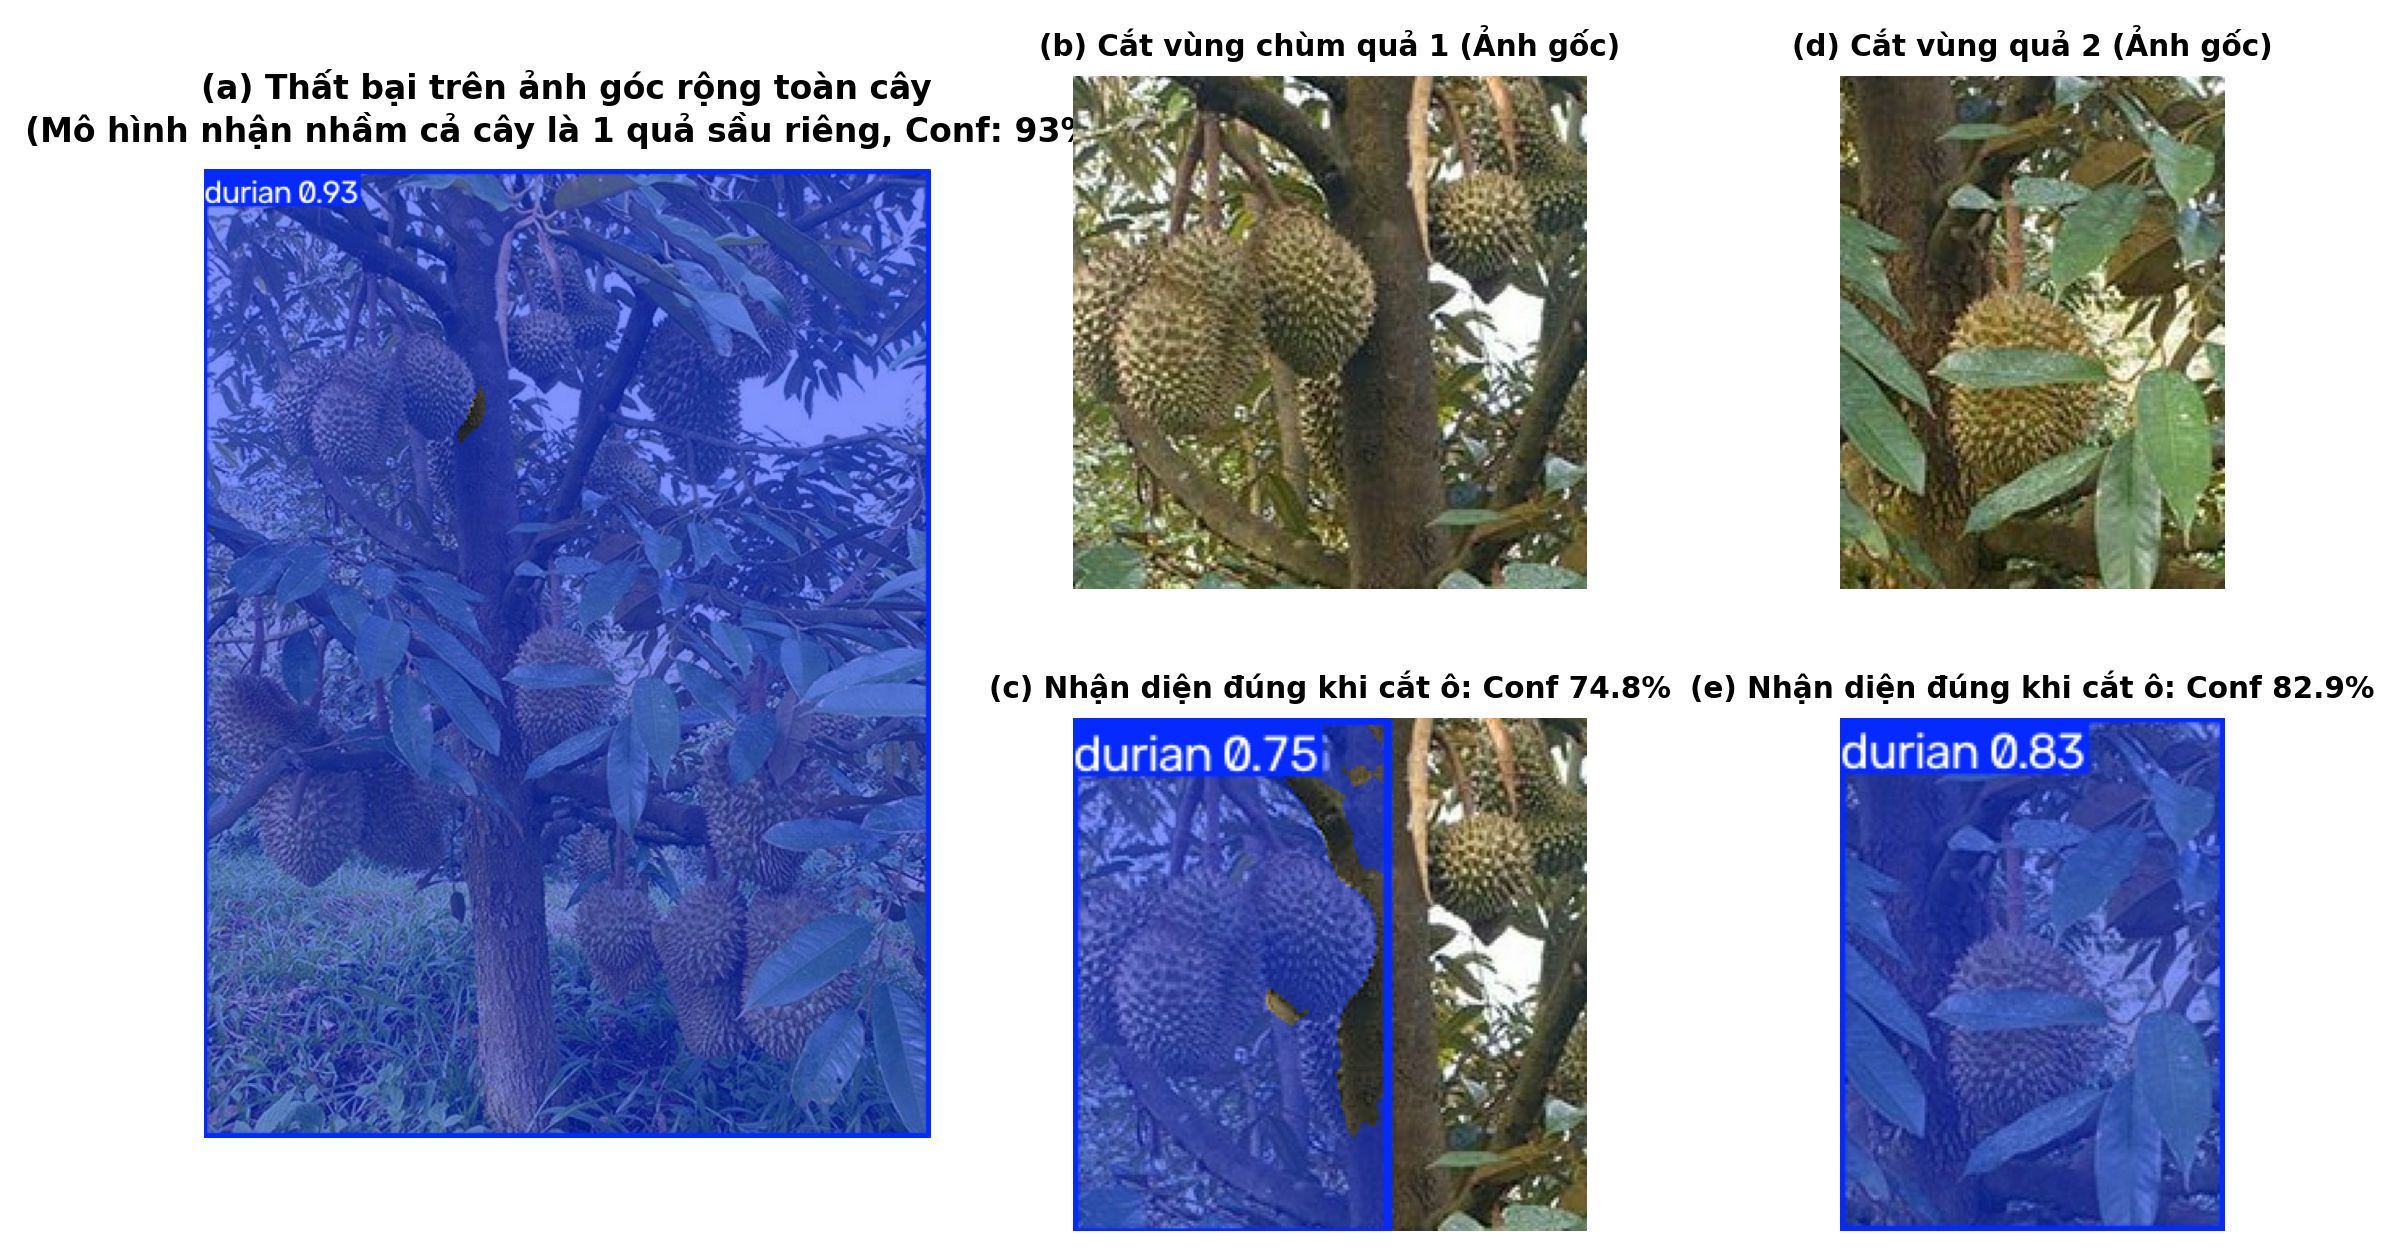
\includegraphics[width=0.98\textwidth]{scale_failure_analysis.png}
}{
    \framebox[0.98\textwidth]{\rule{0pt}{7.0cm} \textbf{HÌNH 3.1: PHÂN TÍCH CA LỖI SUY BIẾN QUY MÔ (scale\_failure\_analysis.png)}}
}
\caption{Phân tích thực nghiệm ca lỗi suy biến quy mô và overfitting trên ảnh vườn tự nhiên (\texttt{sau-rieng2.jpg}). (a) Mô hình nhận diện nhầm toàn bộ tán cây thành 1 quả sầu riêng lớn trùm kín $99.58\%$ diện tích ảnh ($conf = 92.56\%$). (b--c) Cắt ô cụm quả 1: mô hình nhận diện sai lệch khi gộp dính 2 quả làm 1 ($conf = 74.8\%$) và bỏ sót hoàn toàn quả thứ 3 bên phải. (d--e) Cắt ô vùng quả 2: mô hình dự đoán hộp bao trùm kín gần $100\%$ ô cắt ($conf = 82.9\%$), mặt nạ bị rò rỉ nghiêm trọng (boundary bleeding) lên cả thân cây và cành lá xung quanh.}
\label{fig:scale_failure}
\end{figure}

\paragraph{Kiểm toán nguyên nhân gốc rễ (Root Cause Audit):}
Kiểm tra cấu trúc nhãn của 2,676 ảnh huấn luyện đã bộc lộ nguyên nhân sâu xa:
\begin{enumerate}
    \item \textbf{Thiên kiến kích thước cực đoan trong tập dữ liệu (Extreme Scale Bias):} Thống kê toàn bộ tập huấn luyện cho thấy số đối tượng trung bình trên mỗi ảnh chỉ đạt đúng $1.00$ quả/ảnh. Tỷ lệ diện tích của quả sầu riêng chiếm trung bình $30.2\%$ khung hình, và không có bất kỳ ảnh nào chụp toàn cảnh cả cây từ cự ly xa với các quả nhỏ chiếm $1\text{--}2\%$ diện tích. Mạng học sâu bị ép học một tiên nghiệm rằng sầu riêng luôn là một vật thể lớn choán phần lớn khung hình.
    \item \textbf{Trùng lặp ngữ cảnh khung hình video (Contextual Overfitting):} Một lượng lớn ảnh nguồn được trích xuất từ các chuỗi video liên tục (\texttt{frame\_0}, \texttt{frame\_10}, \texttt{frame\_20}...). Mạng nơ-ron học thuộc lòng cấu trúc màu sắc xanh rêu và bề mặt sần sùi chiếm trọn khung hình. Khi gặp tán cây toàn cảnh có màu sắc và kết cấu gồ ghề tương tự, trường tiếp nhận lớn của mạng nhầm lẫn toàn bộ cây là một quả khổng lồ.
    \item \textbf{Ảo tưởng độ chính xác trên tập Validation (Validation Metric Illusion):} Điểm số Mask mAP@50 cao chót vót ($0.9820$) đạt được là do tập validation được chia ngẫu nhiên từ cùng 5 kho dữ liệu cận cảnh. Kết quả này phản ánh chân thực nguy cơ của việc đánh giá mô hình purely trên dữ liệu nội bộ mà thiếu kiểm thử ngoài phân phối (Out-of-Distribution -- OOD).
\end{enumerate}

\paragraph{Phân tích kiểm chứng đối chứng cắt ô: Bộc lộ bản chất Overfitting sâu sắc:}
Khi tiến hành cắt các ô nhỏ xung quanh vùng quả trên ảnh \texttt{sau-rieng2.jpg} nhằm đưa kích thước quả về tỷ lệ tương đồng với tập huấn luyện ($20\%\text{--}30\%$ khung hình), kết quả thực nghiệm tại Hình~\ref{fig:scale_failure}(b--e) đã bộc lộ rõ ràng các khiếm khuyết cốt lõi của mô hình:
\begin{itemize}
    \item \textbf{Tại ô cắt chùm quả 1 (Hình~\ref{fig:scale_failure}c):} Vùng cắt thực tế có 3 quả sầu riêng (chùm 2 quả bên trái và 1 quả đơn bên phải). Mô hình chỉ dự đoán một hộp bao duy nhất gộp dính cả 2 quả bên trái thành một đối tượng (\texttt{durian 0.75}), đồng thời bỏ sót hoàn toàn quả thứ 3 bên phải (False Negative). Điều này chứng minh mô hình bị suy thoái năng lực phân đoạn thực thể riêng biệt (under-segmentation / instance clumping) khi các quả mọc san sát nhau trong chùm tự nhiên.
    \item \textbf{Tại ô cắt quả 2 (Hình~\ref{fig:scale_failure}e):} Quả sầu riêng nằm xen giữa tán lá và thân cây. Mô hình dự đoán một hộp bao trùm kín gần $100\%$ toàn bộ ô cắt (\texttt{durian 0.83}), kéo theo mặt nạ phân đoạn rò rỉ nghiêm trọng (boundary bleeding) lên cả thân cây và lá cây xung quanh. Hiện tượng này khẳng định mạng bị thiên kiến ``chiếm trọn khung hình'' (crop-filling bias): cứ đưa ô nào vào là mạng ép dự đoán một hộp bao choán hết diện tích ô đó mà không phân biệt được ranh giới thực giữa vỏ quả và vỏ cây.
\end{itemize}
Những phát hiện thực nghiệm này khẳng định rằng: \textbf{Mô hình hiện tại đã bị overfitting nặng vào tập dữ liệu ảnh chụp cận cảnh đơn lẻ}, và kỹ thuật cắt ô SAHI thuần túy sẽ không thể khắc phục triệt để nếu mô hình nền tảng chưa được học các đặc trưng trong môi trường tự nhiên thực tế.

\noindent\textbf{Định hướng khắc phục triệt để cho Sprint 4:}
\begin{enumerate}
    \item \textbf{Thu thập bộ dữ liệu thực địa ngoài tự nhiên (In-situ Orchard Dataset):} Bổ sung tối thiểu 300--500 ảnh chụp toàn cảnh tán cây và cự ly trung bình (chụp tại vườn sầu riêng thực tế hoặc nguồn tư liệu thực địa mở) với đa dạng cự ly ($0.5\text{--}5.0\,\text{m}$), mật độ chùm quả phức tạp, quả bị che khuất và điều kiện ánh sáng tự nhiên khác nhau.
    \item \textbf{Giải quyết bài toán gán nhãn tự động bằng Foundation Model (Grounded-SAM):} Nhằm loại bỏ rào cản gán nhãn đa giác thủ công tốn kém hàng trăm giờ công, nhóm sẽ ứng dụng quy trình gán nhãn bán tự động tiên tiến: Sử dụng mô hình nhận diện zero-shot \textbf{Grounding DINO} \cite{liu2023grounding} kết hợp với mô hình nền móng phân đoạn \textbf{Segment Anything (SAM / SAM 2)} \cite{kirillov2023segment}. Văn bản gợi ý (text prompt \texttt{``durian fruit''}) sẽ định hướng Grounding DINO trích xuất bounding box thô, sau đó SAM tự động mở rộng và ôm khít viền gai để sinh nhãn đa giác chuẩn xác cấp pixel. Con người chỉ đóng vai trò kiểm toán và xác nhận nhanh (Human-in-the-loop verification), giúp tăng năng suất tạo dữ liệu lên gấp $20\text{--}30$ lần mà không cần vẽ thủ công từng đỉnh.
    \item \textbf{Tăng cường dữ liệu Copy-Paste và Fine-tune trên SAHI:} Áp dụng kỹ thuật \textit{Instanced Scale Copy-Paste} để dán ngẫu nhiên các quả sầu riêng ở các tỷ lệ nhỏ ($0.05\text{--}0.25$) vào các ảnh nền cây thực tế, sau đó tái huấn luyện mô hình YOLOv8n-seg kết hợp thuật toán suy luận đa tỷ lệ SAHI \cite{akyon2022sahi}.
\end{enumerate}

\subsubsection{Các hạn chế phần cứng và pháp lý khác}
\begin{enumerate}
    \item \textbf{Hiện tượng lóa hồng ngoại do bức xạ mặt trời (Solar IR Washout) trên RealSense D453i:}
    Cảm biến Intel RealSense D453i sử dụng công nghệ stereo hồng ngoại chủ động (active IR stereo) kết hợp máy chiếu hoa văn laser hồng ngoại. Dưới ánh nắng nhiệt đới gay gắt ban ngày, mật độ bức xạ hồng ngoại tự nhiên từ mặt trời lấn át hoa văn chiếu, dẫn đến hiện tượng khuyết thiếu dữ liệu độ sâu (depth holes / dropouts) tại các vùng bề mặt quả bị ánh nắng chiếu trực diện. Trong Sprint 4, nhóm sẽ tích hợp kính lọc phân cực quang học và triển khai thuật toán nội suy điểm ảnh chiều sâu (depth spatial hole-filling) giới hạn nghiêm ngặt bên trong mặt nạ $M(u, v)$ của quả sầu riêng.
    
    \item \textbf{Rung chấn cơ khí khi robot di chuyển trên địa hình đồi dốc:}
    Mặt đường đất gồ ghề, sỏi đá và rãnh thoát nước vườn sầu riêng tạo ra dao động cơ học tần số cao truyền lên khung gầm UGV. Rung chấn gây ra hiện tượng mờ nhòe do chuyển động (motion blur) trên ảnh màu và làm sai lệch pha thời gian giữa khung hình RGB và khung hình độ sâu của RealSense D453i cũng như dữ liệu quét của LiDAR C1M1. Giải pháp kỹ thuật là trang bị cụm giảm chấn cao su giảm rung đa hướng cho cụm cảm biến, đồng thời khai thác dữ liệu từ cảm biến quán tính IMU 6 bậc tự do tích hợp sẵn trên RealSense D453i để bù trừ góc nghiêng động học.
    
    \item \textbf{Ràng buộc bản quyền phần mềm (AGPL-3.0 so với Tự chủ Sản phẩm Doanh nghiệp):}
    Thư viện Ultralytics YOLOv8 được phát hành theo giấy phép GNU Affero General Public License v3.0 (AGPL-3.0), đòi hỏi mã nguồn của các phần mềm liên kết phải mở công khai. Đối với sản phẩm robot nông nghiệp thương mại hóa của doanh nghiệp tài trợ, đây là một ràng buộc pháp lý quan trọng. Nhóm giải quyết triệt để vấn đề này bằng kiến trúc phân tách độc lập: Ultralytics chỉ được sử dụng ngoại tuyến (offline) trên máy trạm trong pha huấn luyện; sau đó, trọng số mô hình được chuyển đổi sang định dạng chuẩn mở ONNX. Trên máy tính nhúng Raspberry Pi 5, một ROS 2 node suy luận bằng C++ thuần sử dụng ONNX Runtime / NCNN sẽ đọc mô hình, hoàn toàn cô lập mã nguồn điều khiển robot khỏi các ràng buộc của giấy phép AGPL-3.0.
\end{enumerate}
% ==============================================================================
% MỤC 4: KẾ HOẠCH CÔNG VIỆC TIẾP THEO
% ==============================================================================
\section{Kế hoạch công việc tiếp theo (Next Work)}

Bảng~\ref{tab:plan} chi tiết hóa các nhiệm vụ kỹ thuật và kết quả bàn giao dự kiến cho Sprint 4 (từ ngày 26/10 đến 08/11/2026, tương ứng Báo cáo tiến độ số 4).

\begin{table}[htbp]
\centering
\small
\caption{Kế hoạch nhiệm vụ kỹ thuật chi tiết cho giai đoạn 26/10 -- 08/11/2026 (Sprint 4).}
\label{tab:plan}
\begin{tabularx}{\textwidth}{c p{7.0cm} X}
\toprule
\textbf{STT} & \textbf{Nội dung nhiệm vụ kỹ thuật} & \textbf{Sản phẩm bàn giao mục tiêu} \\
\midrule
\textbf{1} & Đóng gói mô hình YOLOv8n-seg và giải thuật MF-3DLoc thành một ROS 2 node độc lập trên nền ROS 2 Jazzy cho Raspberry Pi 5 (16\,GB). & Gói node ROS 2 hoàn chỉnh nhận dữ liệu từ RealSense D453i, tích hợp module cắt ô SAHI giải quyết bài toán cây góc rộng, tối ưu hóa suy luận qua ONNX Runtime / NCNN trên nhân ARM NEON. \\
\addlinespace
\textbf{2} & Hiện thực hóa chuỗi biến đổi tọa độ không gian động TF2 từ hệ trục quang học RealSense D453i sang hệ trục bệ tháp pháo UGV. & Xuất bản topic tọa độ mục tiêu thời gian thực \texttt{/turret/target\_3d\_goal} chứa vectơ không gian $(X_T, Y_T, Z_T)$ gắn cờ tin cậy. \\
\addlinespace
\textbf{3} & Đánh giá kiểm chứng độ chính xác bám mục tiêu vòng kín trong môi trường mô phỏng vườn cây Gazebo độ trung thực cao kết hợp dữ liệu LiDAR C1M1. & Video và biểu đồ mô phỏng Gazebo đo đạc sai số động học ngắm bắn của tháp pháo dưới tác động của rung chấn xe UGV trên sườn đồi. \\
\bottomrule
\end{tabularx}
\end{table}

% ==============================================================================
% MỤC 5: ĐỐI CHIẾU VỚI CHUẨN ĐẦU RA MÔN HỌC CO3133
% ==============================================================================
\section{Đối chiếu với chuẩn đầu ra môn học CO3133}

Bảng~\ref{tab:clo_mapping} đối chiếu các hạng mục kỹ thuật đã hoàn thành trong giai đoạn 12/10 -- 25/10/2026 với các Chuẩn đầu ra (CĐR) của môn học CO3133.

\begin{table}[htbp]
\centering
\small
\caption{Bảng đối chiếu chi tiết các kết quả đạt được với Chuẩn đầu ra môn CO3133.}
\label{tab:clo_mapping}
\begin{tabularx}{\textwidth}{>{\raggedright\arraybackslash}p{6.5cm} c X c}
\toprule
\textbf{Hạng mục công việc đã hoàn thành} & \textbf{Ánh xạ CĐR} & \textbf{Mô tả theo Đề cương môn học} & \textbf{Đánh giá} \\
\midrule
Thực hiện benchmark ablation 5 kịch bản trên RTX 3060 (Bảng~2.1), phân tích hội tụ loss đa nhiệm (Hình~2.1), động lực học tắt mosaic tại Epoch 20, phân rã lỗi ma trận nhầm lẫn và tính khoảng tin cậy Wilson 95\% cho Recall. & \textbf{CĐR 8 (L.O.5.1)} & Vận dụng các chỉ số đo lường định lượng, quy trình ablation và phân rã sai số để đánh giá mô hình học sâu trên tập dữ liệu chuyên ngành. & \textbf{Hoàn thành} \\
\addlinespace
Phân tích đánh đổi kiến trúc (YOLOv8n-seg so với YOLOv8s-seg), đánh đổi độ phân giải và kích thước batch, lập kế hoạch ngân sách tài nguyên CPU/RAM trên Raspberry Pi 5 (16\,GB), camera RealSense D453i và LiDAR C1M1 (Mục~3). & \textbf{CĐR 9 (L.O.5.2)} & Xây dựng luận điểm và chứng minh lựa chọn mô hình kỹ thuật tối ưu thỏa mãn các ràng buộc biên phần cứng (độ trễ, thông lượng, RAM, công suất). & \textbf{Hoàn thành} \\
\addlinespace
Thiết lập, tinh chỉnh và vận hành pipeline huấn luyện trên trạm GPU NVIDIA RTX 3060 sử dụng PyTorch 2.3.0 và Ultralytics 8.2 (Mục~1.3, Mục~2). & \textbf{CĐR 4 (L.O.4.1)} & Hiện thực hóa và huấn luyện các mô hình học sâu hiện đại bằng các thư viện phần mềm chuyên dụng trên hạ tầng phần cứng GPU. & \textbf{Hoàn thành} \\
\addlinespace
Tổng hợp dữ liệu từ 5 kho Roboflow, chuẩn hóa nhãn đa giác về lớp sầu riêng duy nhất qua \texttt{merge\_datasets.py}, sàng lọc dữ liệu lỗi, chia tập độc lập 80/14/6 và áp dụng tăng cường trực tuyến trong bộ nhớ (Mục~2.1). & \textbf{CĐR 5 (L.O.4.2)} & Thiết kế quy trình thu thập, làm sạch, tiền xử lý và tăng cường dữ liệu nhằm bảo toàn tính liêm chính và chống rò rỉ dữ liệu. & \textbf{Hoàn thành} \\
\bottomrule
\end{tabularx}
\end{table}

\newpage
% TÀI LIỆU THAM KHẢO
% ==============================================================================
\begin{thebibliography}{10}

\bibitem{ultralytics2023}
G.~Jocher, A.~Chaurasia, và J.~Kwon, ``Ultralytics YOLOv8,'' 2023. [Trực tuyến]. Địa chỉ: \url{https://github.com/ultralytics/ultralytics}

\bibitem{zheng2020ciou}
Z.~Zheng, P.~Wang, W.~Liu, J.~Li, R.~Ye, và D.~Ren, ``Distance-IoU loss: Faster and better learning for bounding box regression,'' trong \textit{Kỷ yếu Hội nghị Quốc tế AAAI về Trí tuệ Nhân tạo}, tập~34, số~07, 2020, tr. 12\,993--13\,000.

\bibitem{li2020generalized}
X.~Li, C.~Lv, W.~Wang, G.~Li, L.~Yang, và J.~Yang, ``Generalized focal loss: Learning qualified and distributed bounding boxes for dense object detection,'' trong \textit{Hội nghị Quốc tế về Hệ thống Xử lý Thông tin Nơ-ron (NeurIPS)}, tập~33, 2020, tr. 21\,002--21\,012.

\bibitem{macenski2020marathon}
S.~Macenski, F.~Mart{\'\i}n, R.~White, và J.~Gin{\'e}s Clavero, ``The Marathon 2: A navigation system,'' trong \textit{Hội nghị Quốc tế IEEE/RSJ về Robot Thông minh và Hệ thống (IROS)}, 2020, tr. 2718--2725.

\bibitem{he2017maskrcnn}
K.~He, G.~Gkioxari, P.~Doll{\'a}r, và R.~Girshick, ``Mask R-CNN,'' trong \textit{Hội nghị Quốc tế IEEE/CVF về Thị giác Máy tính (ICCV)}, 2017, tr. 2961--2969.

\bibitem{bolya2019yolact}
D.~Bolya, C.~Zhou, F.~Xiao, và Y.~J.~Lee, ``YOLACT: Real-time instance segmentation,'' trong \textit{Hội nghị Quốc tế IEEE/CVF về Thị giác Máy tính (ICCV)}, 2019, tr. 9157--9166.

\bibitem{wilson1927probable}
E.~B.~Wilson, ``Probable inference, the law of succession, and statistical inference,'' \textit{Tạp chí của Hiệp hội Thống kê Hoa Kỳ (Journal of the American Statistical Association)}, tập~22, số~158, tr. 209--212, 1927.

\bibitem{fu2020rgbd}
L.~Fu, F.~Gao, J.~Wu, R.~Li, M.~Karkee, và Q.~Zhang, ``Application of consumer RGB-D cameras for fruit detection and localization in field: A critical review,'' \textit{Computers and Electronics in Agriculture}, tập~177, tr. 105687, 2020. [Trực tuyến]. DOI: \url{https://doi.org/10.1016/j.compag.2020.105687}

\bibitem{lin2021fruit}
G.~Lin, Y.~Tang, X.~Zou, và C.~Wang, ``Three-dimensional reconstruction of fruits and branches using instance segmentation and geometry analysis,'' \textit{Computers and Electronics in Agriculture}, tập~184, tr. 106107, 2021. [Trực tuyến]. DOI: \url{https://doi.org/10.1016/j.compag.2021.106107}

\bibitem{kang2020dasnet}
H.~Kang và C.~Chen, ``Fruit detection, segmentation and 3D visualisation of environments in apple orchards,'' \textit{Computers and Electronics in Agriculture}, tập~171, tr. 105302, 2020. [Trực tuyến]. DOI: \url{https://doi.org/10.1016/j.compag.2020.105302}

\bibitem{akyon2022sahi}
F.~C.~Akyon, S.~O.~Altinuc, và A.~Temizel, ``Slicing Aided Hyper Inference and fine-tuning for small object detection,'' trong \textit{Hội nghị Quốc tế IEEE về Xử lý Ảnh (ICIP)}, 2022, tr. 966--970. [Trực tuyến]. DOI: \url{https://doi.org/10.1109/ICIP46576.2022.9897990}

\bibitem{kirillov2023segment}
A.~Kirillov, E.~Mintun, N.~Ravi, H.~Mao, C.~Rolland, L.~Gustafson, T.~Xiao, S.~Whitehead, A.~C.~Berg, W.-Y.~Lo, P.~Doll{\'a}r, và R.~Girshick, `Segment anything,'' trong \textit{Kỷ yếu Hội nghị Quốc tế IEEE/CVF về Thị giác Máy tính (ICCV)}, 2023, tr. 4015--4026. [Trực tuyến]. DOI: \url{https://doi.org/10.1109/ICCV51070.2023.00371}

\bibitem{liu2023grounding}
S.~Liu, Z.~Zeng, T.~Ren, F.~Li, H.~Zhang, J.~Yang, C.~Li, J.~Yang, H.~Su, J.~Zhu, và L.~Zhang, `Grounding DINO: Marrying DINO with grounded pre-training for open-set object detection,'' trong \textit{Kỷ yếu Hội nghị Châu Âu về Thị giác Máy tính (ECCV)}, 2024. [Trực tuyến]. arXiv:2303.05499.
\end{thebibliography}

\end{document}
\subsubsection{Ca kiểm chứng chùm quả \texttt{sau-rieng3.jpg}: Hiện tượng bỏ sót cá thể do che khuất và chồng lấn}
Để kiểm chứng phản ứng của mô hình khi gặp chùm quả ngoài tự nhiên, nhóm đã chạy suy luận trên ảnh thực tế \texttt{sau-rieng3.jpg}. Khung hình này chứa một chùm gồm \textbf{3 quả sầu riêng mọc sát nhau và nằm đè chồng lấn lên nhau}:
\begin{itemize}
    \item \textbf{Kết quả thực nghiệm:} Mô hình chỉ phát hiện được \textbf{đúng 1 quả nổi bật nhất ở phía trước} với độ tin cậy $91.79\%$ (hộp bao $[164.1, 118.1, 702.3, 395.7]$ chiếm $31.13\%$ diện tích ảnh), trong khi \textbf{2 quả sầu riêng mọc phía sau bị bỏ sót hoàn toàn (False Negatives)}!
    \item \textbf{Bản chất và Nguyên nhân gốc rễ:}
    \begin{enumerate}
        \item \textit{Thiên lệch dữ liệu đơn lẻ (Single-Fruit Bias):} Tập dữ liệu Roboflow huấn luyện gồm 1,053 ảnh hầu hết là các quả đơn lẻ mọc biệt lập (trung bình chỉ $1.2$ quả/ảnh). Mạng nơ-ron chưa từng được học cách phân tách các chùm quả dày đặc mọc đè lên nhau.
        \item \textit{Đồng nhất hóa kết cấu bề mặt gai (Texture Homogenization):} Cả 3 quả đều có bề mặt gai màu nâu xanh tương đồng. Tại ranh giới tiếp xúc giữa hai quả không có độ tương phản màu sắc lớn, khiến các tầng tích chập coi cụm gai liền kề là thuộc về quả lớn phía trước.
        \item \textit{Triệt tiêu của thuật toán NMS (Non-Maximum Suppression):} Do hai quả phía sau nằm trùng vị trí không gian với quả phía trước, các đề xuất hộp bao của chúng có IoU cao với quả chính, dẫn đến việc bị thuật toán NMS mặc định ($\text{IoU} = 0.7$) triệt tiêu.
    \end{enumerate}
    \item \textbf{Giải pháp cho Sprint 4:} Áp dụng kỹ thuật tăng cường tổng hợp Copy-Paste đè quả với tỷ lệ ngẫu nhiên ($30\text{--}70\%$), chuyển sang thuật toán \textbf{Soft-NMS} hoặc \textbf{Mask-guided NMS} (dựa trên IoU mặt nạ thay vì hộp bao), và áp dụng cơ chế thị giác chủ động \textbf{Active Multi-view Vision} trên cánh tay robot (xoay camera $\pm 25^\circ$ để bóc tách quả bằng đám mây điểm chiều sâu 3D).
\end{itemize}


